\documentclass[preprint,review,12pt]{elsarticle}

% Allow Computer Modern fonts to scale to the sizes produced when wide
% tables are fitted with adjustbox.
\usepackage{fix-cm}
\usepackage[T1]{fontenc}
\usepackage{lmodern}
\usepackage{amsmath,amssymb,amsfonts}
\usepackage{graphicx}
\usepackage{adjustbox}
\usepackage{booktabs}
\usepackage{multirow}
\usepackage{algorithm}
\usepackage{algpseudocode}
\usepackage{url}
\usepackage[hidelinks,bookmarks=false]{hyperref}
\usepackage{orcidlink}
% Applied Soft Computing uses numbered citations for this submission.
\biboptions{numbers,sort&compress}

\graphicspath{{figures/}}
\emergencystretch=3em
\journal{Applied Soft Computing}

\begin{document}
\begin{frontmatter}

\title{WindFormer: A Common-Speed and Direction-Vector Network for Wind Resource Forecasting}

\author[inst1]{Junhua Chai\orcidlink{0009-0000-2910-4661}}
\author[inst1]{Rui Zhou\orcidlink{0009-0004-7055-5359}}
\ead{18318582708@163.com}
\author[inst1]{Huazhou Chen\orcidlink{0000-0003-4770-020X}}
\author[inst1]{Quanxi Feng\orcidlink{0000-0002-7720-4453}}
\ead{fqx9904@163.com}
\address[inst1]{School of Mathematics and Statistics, Guilin University of Technology, Guilin, China. Corresponding authors: Rui Zhou and Quanxi Feng.}

\begin{abstract}
Accurate short-term wind resource forecasting is critical for wind farm dispatch and power system operation, yet wind speed and wind direction exhibit different cross-turbine structures and mathematical properties. Wind speed combines shared meteorological evolution with turbine-level deviations, whereas wind direction is turbine-specific and circular, making a single homogeneous interaction pattern inadequate. We propose WindFormer, a structure-aware dual-branch network that extracts a learnable common wind-speed field, models turbine residuals with shared predictors, and organizes the common history using Phase-Attention over screened candidate temporal scales. In parallel, WindFormer forecasts each turbine's wind direction in a continuous sine-cosine vector space with shared Patch-Attention, and couples the two branches through a physical wind-vector consistency objective. Experiments on two public wind-farm datasets show consistent improvements over the compared forecasting baselines across wind-speed and wind-direction metrics and forecast horizons. Component ablations, matched-seed statistical tests, perturbation and extreme-volatility stress tests, efficiency measurements, and sparse-deployment zero-shot experiments further examine the mechanism, stability, computational cost, and cross-turbine generalization of the proposed framework.
\end{abstract}

\begin{keyword}
Spatio-temporal modeling \sep wind speed forecasting \sep wind direction forecasting \sep wind turbines \sep deep learning \sep time series forecasting
\end{keyword}
\end{frontmatter}

\section{Introduction}
\label{sec:introduction}

Driven by its clean nature and reliable supply, wind power has become an important energy source for modern power systems. Accurate short-term forecasts of wind speed and wind direction support grid dispatch, resource allocation, and wind-energy utilization \cite{Hanifi2020CriticalReviewWindPowerForecasting,Jung2014CurrentStatusWindSpeedPowerForecasting}. In a wind farm, however, these variables are not homogeneous multivariate channels. They are shaped by different physical structures across turbines and also have different mathematical properties \cite{Chen2014WindPowerForecastsGaussianProcesses,Dolatabadi2022DeepSpatialTemporal2DCNNBLSTM}. A forecasting model should therefore share information selectively rather than imposing one interaction pattern on every wind variable.

\begin{figure}[htbp]
\centering

\includegraphics[width=0.9\textwidth]{figures/figure1.png}
\caption{Conceptual contrast between shared but non-identical wind-speed dynamics and turbine-specific wind-direction variation.}
\label{fig:data_properties}
\end{figure}

\subsection{Challenge 1: Shared but Non-identical Wind-Speed Dynamics}
\label{subsec:speed_sharing_intro}

Wind turbines in the same farm are driven by common weather processes and large-scale incoming flows, so their wind-speed trajectories often exhibit synchronized trends. At the same time, local terrain, wake effects, and turbine positions produce turbine-level deviations. This combination creates a structural tension: channel-independent methods preserve local freedom but repeatedly relearn common variation, whereas fully correlated methods may mix common dynamics and local deviations in a single representation. The key challenge is therefore to share the common wind field while retaining turbine-specific residual information.

Figure~\ref{fig:speed_multiscale_similarity} provides supporting evidence for this view. Representative turbines exhibit similar dominant spectral components and wavelet-energy patterns, suggesting a shared temporal scaffold rather than a collection of unrelated sequences. The remaining differences motivate a separate residual branch instead of assuming that all turbines are identical.

\begin{figure}[htbp]
\centering
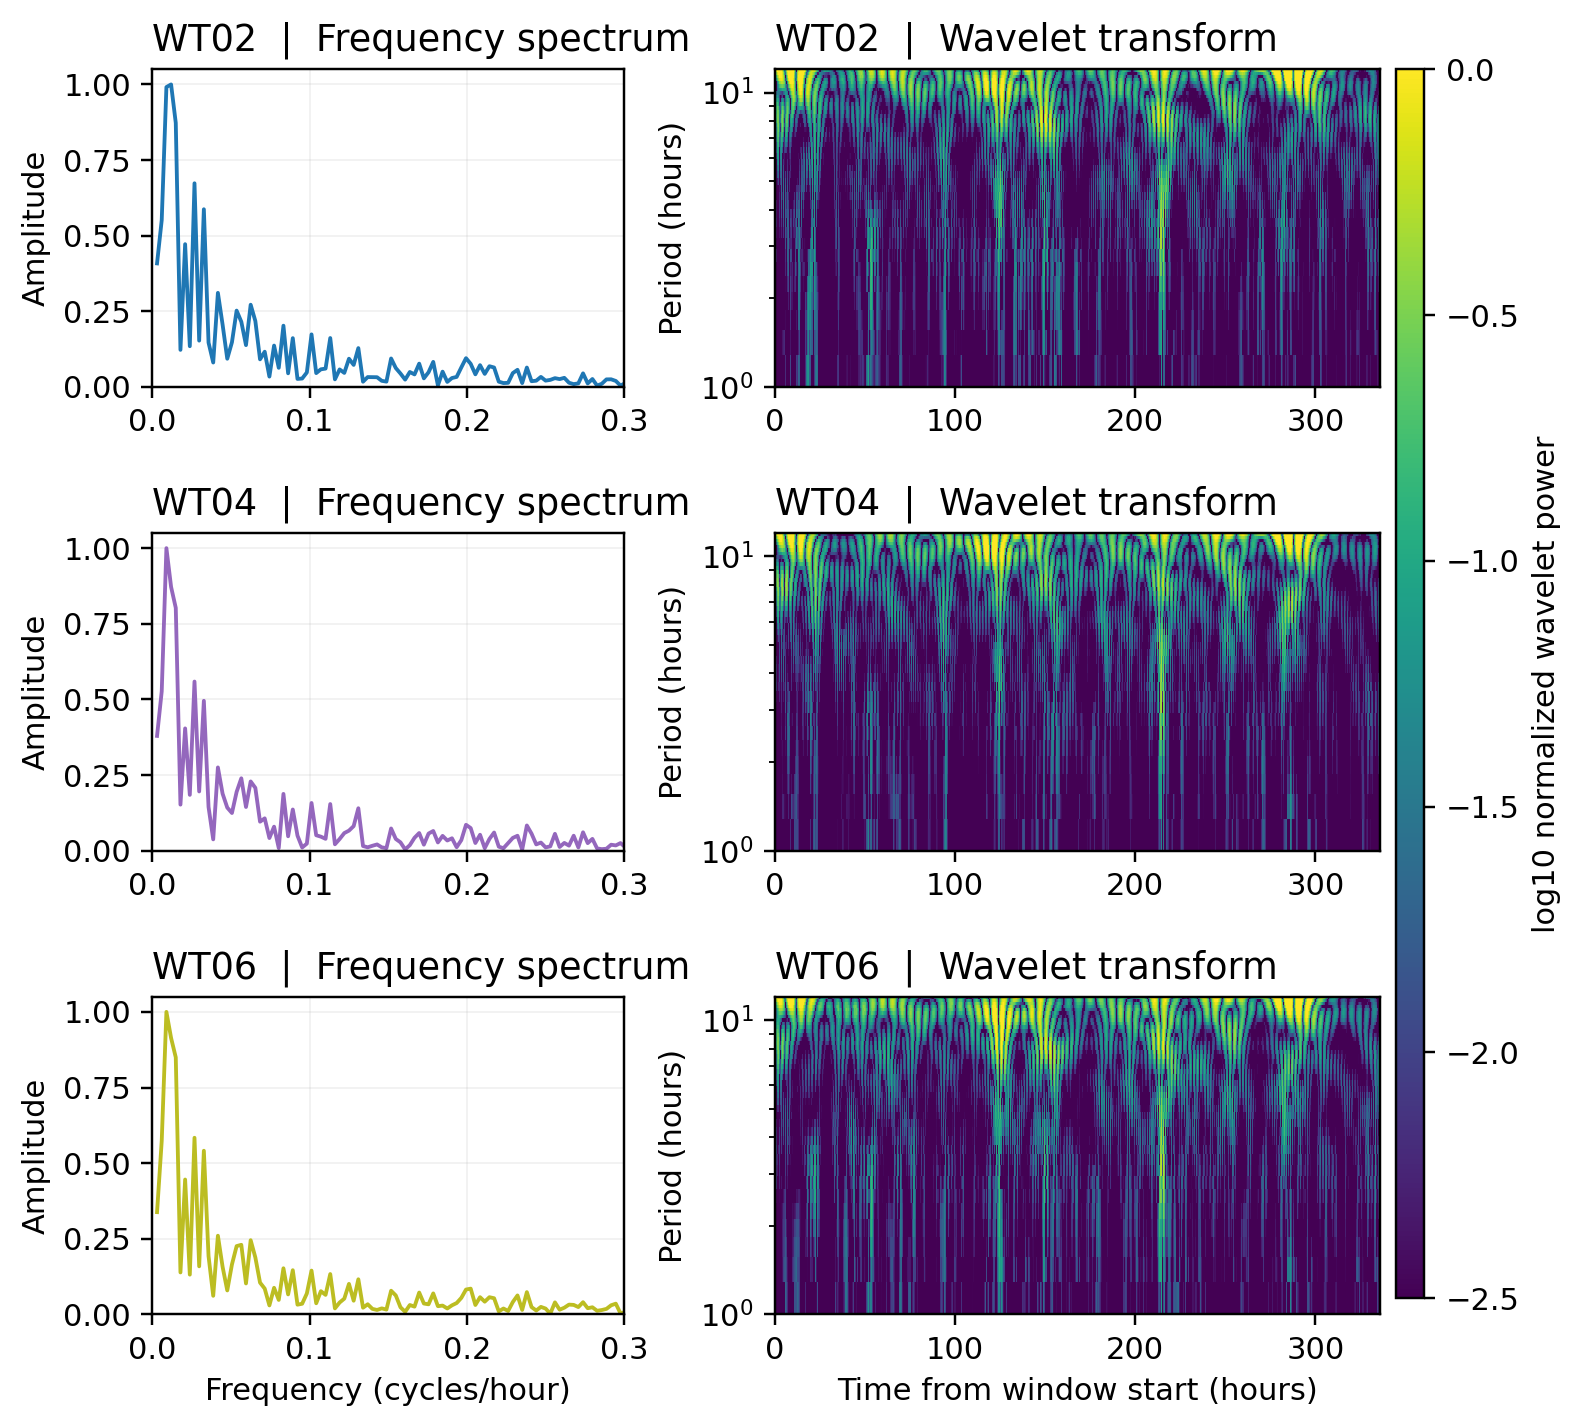
\includegraphics[width=0.9\textwidth]{figures/figure2.png}
\caption{Frequency-spectrum and wavelet-transform comparison of representative turbine wind-speed sequences. Similar dominant components support a shared temporal scaffold, while turbine-level deviations motivate residual modeling.}
\label{fig:speed_multiscale_similarity}
\end{figure}

After separating the shared component, the common wind-speed history still needs an effective temporal organization. Rather than treating a screened candidate scale as a strict physical period, we organize the history by candidate temporal scales and relative phase positions within temporal blocks. This phase-aware organization allows local dynamics at comparable positions across blocks to interact.

\subsection{Challenge 2: Turbine-specific and Circular Wind Directions}
\label{subsec:direction_2d_intro}

Wind direction follows a different cross-turbine structure. Interactions among turbine locations, wake effects, and local flow fields cause different units to exhibit distinct dominant directions and turning patterns, so direction should not be collapsed into a common representation in the same way as wind speed. Figure~\ref{fig:direction_specificity} (a) shows that the dominant directions and directional concentration levels of different turbines are not consistent. Figure~\ref{fig:direction_specificity} (b) reports that about 51\% of turbine pairs have an average angular distance of no less than $90^\circ$, indicating that the heterogeneity is not caused by a few isolated units. Figure~\ref{fig:direction_specificity} (c) further displays structured variation in the pairwise angular-distance matrix. These observations motivate turbine-wise direction modeling.

\begin{figure}[htbp]
\centering

\includegraphics[width=0.9\textwidth]{figures/all_24_turbines_direction_difference_summary.png}
\caption{Turbine-specific wind-direction distributions and all-pair angular differences among 24 turbines.}
\label{fig:direction_specificity}
\end{figure}

Wind direction is also a circular variable rather than an ordinary one-dimensional scalar. It satisfies

\begin{equation}
\theta \equiv \theta+360^\circ.
\end{equation}

Consequently, $359^\circ$ and $1^\circ$ are physically close even though their scalar difference is $358^\circ$. Direct scalar regression can therefore create artificial discontinuities in distances, local variations, and error gradients. To preserve this geometry from input to prediction, WindFormer maps each direction angle into a two-dimensional sine-cosine unit vector:

\begin{equation}
\mathbf{u}_{t,n} = [\cos(\theta_{t,n}), \sin(\theta_{t,n})].
\end{equation}

The model predicts in this continuous representation, applies direction-vector and wind-vector consistency constraints, and recovers the angle using

\begin{equation}
\hat{\theta}_{t,n} = \operatorname{atan2} \left( \hat{u}^{\sin}_{t,n}, \hat{u}^{\cos}_{t,n} \right).
\end{equation}

Because directional patterns remain turbine-specific, each turbine is processed as an individual two-dimensional sequence. The temporal patch projection and Patch-Attention encoder are shared across turbines, allowing transferable local dynamics to be learned without collapsing distinct directional distributions into one global state.

\subsection{WindFormer Framework}

The two challenges lead to a single design principle: share information where the wind field is physically common, preserve information where turbine behavior is specific, and keep the direction representation geometrically valid. WindFormer implements this principle with two representation-decoupled branches and one objective-level coupling mechanism. The wind-speed branch extracts a learnable common field, models it with Phase-Attention organized by screened candidate temporal scales, and reconstructs turbine forecasts from the common prediction and shared residual predictors. The wind-direction branch retains each turbine's sequence, maps angles to sine-cosine components, and uses shared Patch-Attention to forecast future direction vectors. The branches are trained jointly through wind-speed, direction-vector, and wind-vector consistency losses.

The main contributions of this paper are as follows:

\begin{itemize}
    \item \textbf{We separate shared and local wind-speed dynamics.} A learnable aggregation extracts shared wind-speed dynamics, while a shared residual branch restores turbine-level deviations. A phase-aware temporal encoder organizes the common history by screened candidate scales and relative positions rather than assuming a strict physical period.
    \item \textbf{We develop a turbine-wise circular direction branch within the same forecasting framework.} Sine-cosine vectors preserve boundary continuity, and shared Patch-Attention captures transferable temporal patterns while retaining turbine-specific directional sequences.
    \item \textbf{We couple the two task-specific branches through a physical wind-vector objective and evaluate the resulting WindFormer framework comprehensively.} Standard forecasting, component ablations, robustness tests, sparse-deployment transfer, efficiency measurements, and matched-seed statistical tests together assess accuracy, mechanism, stability, and generalization.
\end{itemize}

\section{Related Work}
\label{sec:related_work}

\subsection{Spatial Relationships in Multi-Turbine Wind Power Forecasting}

Existing deep learning studies usually improve wind forecasting by modeling spatial relationships among turbines. Graph-based and convolutional recurrent models encode turbine topology, neighborhood influence, multi-scale spatial dependence, or local and long-range interactions into the forecasting process \cite{Song2023ShortTermForecastingGraphConvolutionWindPower,Zhang2019LSTMNeighborhoodGatesCausalityWindSpeed,Wu2024MixFormerHierarchicalContextWindSpeed}. To handle condition-dependent relationships, later studies further introduce channel-aware dependence and temporal lead-lag structures \cite{Zhao2024RethinkingChannelDependenceLeadingIndicators,Zhu2024GGNetTemporalLeadLagCorrelations}. These methods show that cross-turbine information is useful for short-term wind forecasting.

Generic multivariate time-series models also provide useful designs for organizing turbine variables. PatchTST reduces cross-channel interference through channel-independent temporal modeling \cite{Nie2023PatchTST}, TimesNet converts temporal variations into two-dimensional period structures \cite{Wu2023TimesNetTemporal2DVariationModeling}, iTransformer learns dependencies along the variable dimension \cite{Liu2024iTransformer}, and MSGNet enhances multi-scale cross-sequence interaction \cite{Cai2024MSGNetLearningMultiScaleInterSeriesCorrelations}. MST-Net further discusses the combination of channel-independent and spatially correlated modeling for short-term wind resource forecasting \cite{Lou2026MSTNet}. More recently, an Information Sciences study further explores a global-local dual-branch design and pyramid patch interaction for multivariate forecasting \cite{Zhou2026GLPTGlobalLocalPyramidTransformer}.

However, most existing methods regard cross-turbine relationships as a single interaction pattern to be learned. They seldom separate the common wind-speed field shared by multiple turbines from turbine-specific residual variations. This distinction is important because wind speeds in the same wind farm often share dominant meteorological trends, while local terrain, wake effects, and turbine positions still introduce individual deviations.

\subsection{Wind Direction Forecasting and Two-Dimensional Representation}

Wind direction forecasting has been studied together with wind speed prediction, yaw-state modeling, and short-term directional change prediction. Representative works include ARMA-based joint wind speed and direction forecasting \cite{Erdem2011ARMATupleWindSpeedDirection}, yaw-error prediction based on wind-direction changes \cite{Ouyang2017PredictiveYawError}, and two-phase deep models designed for short-term wind-direction sequences \cite{Tang2021TwoPhaseWindDirection}.

Unlike wind speed, raw wind direction is a one-dimensional angle with boundary discontinuity. Sine-cosine representations provide a natural way to embed direction angles into a continuous two-dimensional space \cite{Erdem2011ARMATupleWindSpeedDirection,Ouyang2017PredictiveYawError}. Nevertheless, existing studies mainly focus on single direction sequences or general speed-direction joint prediction. Systematic modeling of multi-turbine directional heterogeneity under periodic-boundary constraints remains insufficiently explored.

\input{sections/method}
\section{Experiments}
\label{sec:experiments}

\subsection{Experimental Setup}
\label{subsec:experimental_setup}

We evaluate WindFormer on two SCADA-based wind farm datasets with distinct spatial layouts and wind regimes: Shanxi with 24 turbines and Penmanshiel with 14 turbines. Both datasets are sampled at 10-min intervals and preprocessed following the protocol in Section~\ref{sec:data_preprocessing_task}. Unless otherwise specified, the input window is 288 steps, corresponding to 48 h of history, and the forecasting horizons are 6, 12, and 18 steps.

\begin{figure}[htbp]
\centering

\includegraphics[width=0.8\textwidth]{figures/data.png}
\caption{Geographical visualization of the two wind farm datasets used in the experiments.}
\label{fig:dataset_geography}
\end{figure}

WindFormer is compared with MST-Net, PatchTST, TimeMixer++, GLPT, DLinear, TimesNet, and iTransformer. Mean absolute error (MAE) and root mean squared error (RMSE) are reported for wind speed (m/s) and wind direction (rad). The experiments are organized around four research questions: standard accuracy and efficiency (RQ1), component attribution (RQ2), robustness to perturbations and extreme volatility (RQ3), and transfer to unseen turbines (RQ4).

\subsection{RQ1: Does WindFormer Improve Forecasting Accuracy and Efficiency?}
\label{subsec:standard_forecasting}

The standard setting trains and tests on the full turbine set without artificial perturbation. We first compare the complete forecasting performance on the two wind farms, then examine direction-aware error profiles, computational cost, and matched-seed statistical consistency.

\begin{table}[htbp]
\caption{Detailed full-sample forecasting performance on the Penmanshiel dataset under the noise-free setting. Lower values indicate better performance.}
\label{tab:main_penmanshiel}
\centering
\scriptsize
\setlength{\tabcolsep}{5pt}
\renewcommand{\arraystretch}{1.04}
\begin{adjustbox}{max width=\textwidth}
\begin{tabular}{llcccccccc}
\toprule
Metric & Horizon & WindFormer & MST-Net & TimeMixer++ & iTransformer & PatchTST & TimesNet & GLPT & DLinear \\
\midrule
\multirow{3}{*}{Speed MAE} & 6 & \textbf{0.7142} & 0.7978 & 0.9229 & 0.9272 & 0.9189 & 0.9210 & 0.9318 & 0.9263 \\
& 12 & \textbf{0.8812} & 0.9879 & 1.1421 & 1.1491 & 1.1347 & 1.1406 & 1.1543 & 1.1473 \\
& 18 & \textbf{1.0103} & 1.1249 & 1.2994 & 1.3081 & 1.2891 & 1.2976 & 1.3138 & 1.3061 \\
\midrule
\multirow{3}{*}{Speed RMSE} & 6 & \textbf{1.1497} & 1.2162 & 1.3053 & 1.3118 & 1.2987 & 1.3033 & 1.3174 & 1.3108 \\
& 12 & \textbf{1.4211} & 1.5538 & 1.6162 & 1.6247 & 1.6054 & 1.6142 & 1.6325 & 1.6224 \\
& 18 & \textbf{1.6216} & 1.7599 & 1.8367 & 1.8477 & 1.8263 & 1.8348 & 1.8553 & 1.8447 \\
\midrule
\multirow{3}{*}{Direction MAE} & 6 & \textbf{0.1456} & 0.1637 & 0.1898 & 0.1911 & 0.1884 & 0.1894 & 0.1926 & 0.1939 \\
& 12 & \textbf{0.1881} & 0.2113 & 0.2439 & 0.2460 & 0.2403 & 0.2434 & 0.2483 & 0.2497 \\
& 18 & \textbf{0.2204} & 0.2471 & 0.2847 & 0.2872 & 0.2807 & 0.2840 & 0.2899 & 0.2913 \\
\midrule
\multirow{3}{*}{Direction RMSE} & 6 & \textbf{0.2914} & 0.3092 & 0.3314 & 0.3341 & 0.3294 & 0.3320 & 0.3354 & 0.3375 \\
& 12 & \textbf{0.3686} & 0.3905 & 0.4176 & 0.4213 & 0.4146 & 0.4184 & 0.4237 & 0.4260 \\
& 18 & \textbf{0.4244} & 0.4599 & 0.4796 & 0.4843 & 0.4761 & 0.4807 & 0.4870 & 0.4906 \\
\bottomrule
\end{tabular}
\end{adjustbox}
\end{table}

\begin{table}[htbp]
\caption{Detailed full-sample forecasting performance on the Shanxi dataset under the noise-free setting. Lower values indicate better performance.}
\label{tab:main_shanxi}
\centering
\scriptsize
\setlength{\tabcolsep}{5pt}
\renewcommand{\arraystretch}{1.04}
\begin{adjustbox}{max width=\textwidth}
\begin{tabular}{llcccccccc}
\toprule
Metric & Horizon & WindFormer & MST-Net & TimeMixer++ & iTransformer & PatchTST & TimesNet & GLPT & DLinear \\
\midrule
\multirow{3}{*}{Speed MAE} & 6 & \textbf{0.6367} & 0.7062 & 0.8192 & 0.8222 & 0.8165 & 0.8274 & 0.8270 & 0.8217 \\
& 12 & \textbf{0.8025} & 0.8939 & 1.0343 & 1.0395 & 1.0309 & 1.0452 & 1.0447 & 1.0379 \\
& 18 & \textbf{0.9309} & 1.0337 & 1.1970 & 1.2024 & 1.1953 & 1.2098 & 1.2094 & 1.2013 \\
\midrule
\multirow{3}{*}{Speed RMSE} & 6 & \textbf{0.9884} & 1.0377 & 1.1203 & 1.1248 & 1.1172 & 1.1320 & 1.1311 & 1.1242 \\
& 12 & \textbf{1.2374} & 1.3033 & 1.4035 & 1.4097 & 1.3986 & 1.4178 & 1.4167 & 1.4078 \\
& 18 & \textbf{1.4116} & 1.4862 & 1.6002 & 1.6073 & 1.5987 & 1.6172 & 1.6161 & 1.6059 \\
\midrule
\multirow{3}{*}{Direction MAE} & 6 & \textbf{0.2717} & 0.2984 & 0.3460 & 0.3478 & 0.3445 & 0.3507 & 0.3500 & 0.3516 \\
& 12 & \textbf{0.3441} & 0.3806 & 0.4403 & 0.4426 & 0.4384 & 0.4465 & 0.4459 & 0.4476 \\
& 18 & \textbf{0.4019} & 0.4437 & 0.5130 & 0.5160 & 0.5115 & 0.5206 & 0.5199 & 0.5223 \\
\midrule
\multirow{3}{*}{Direction RMSE} & 6 & \textbf{0.5530} & 0.5778 & 0.6225 & 0.6269 & 0.6210 & 0.6283 & 0.6273 & 0.6300 \\
& 12 & \textbf{0.6525} & 0.7041 & 0.7356 & 0.7409 & 0.7342 & 0.7454 & 0.7440 & 0.7471 \\
& 18 & \textbf{0.7275} & 0.7831 & 0.8196 & 0.8255 & 0.8184 & 0.8295 & 0.8285 & 0.8324 \\
\bottomrule
\end{tabular}
\end{adjustbox}
\end{table}

Tables~\ref{tab:main_penmanshiel} and \ref{tab:main_shanxi} show that WindFormer achieves the best wind-speed and wind-direction accuracy across all reported horizons on both datasets. The consistent ranking across terrain conditions and forecast lengths supports the central design choice of matching the representation to the physical structure of each variable.

\begin{figure}[htbp]
\centering
\setlength{\tabcolsep}{0pt}
\begin{tabular}{cc}
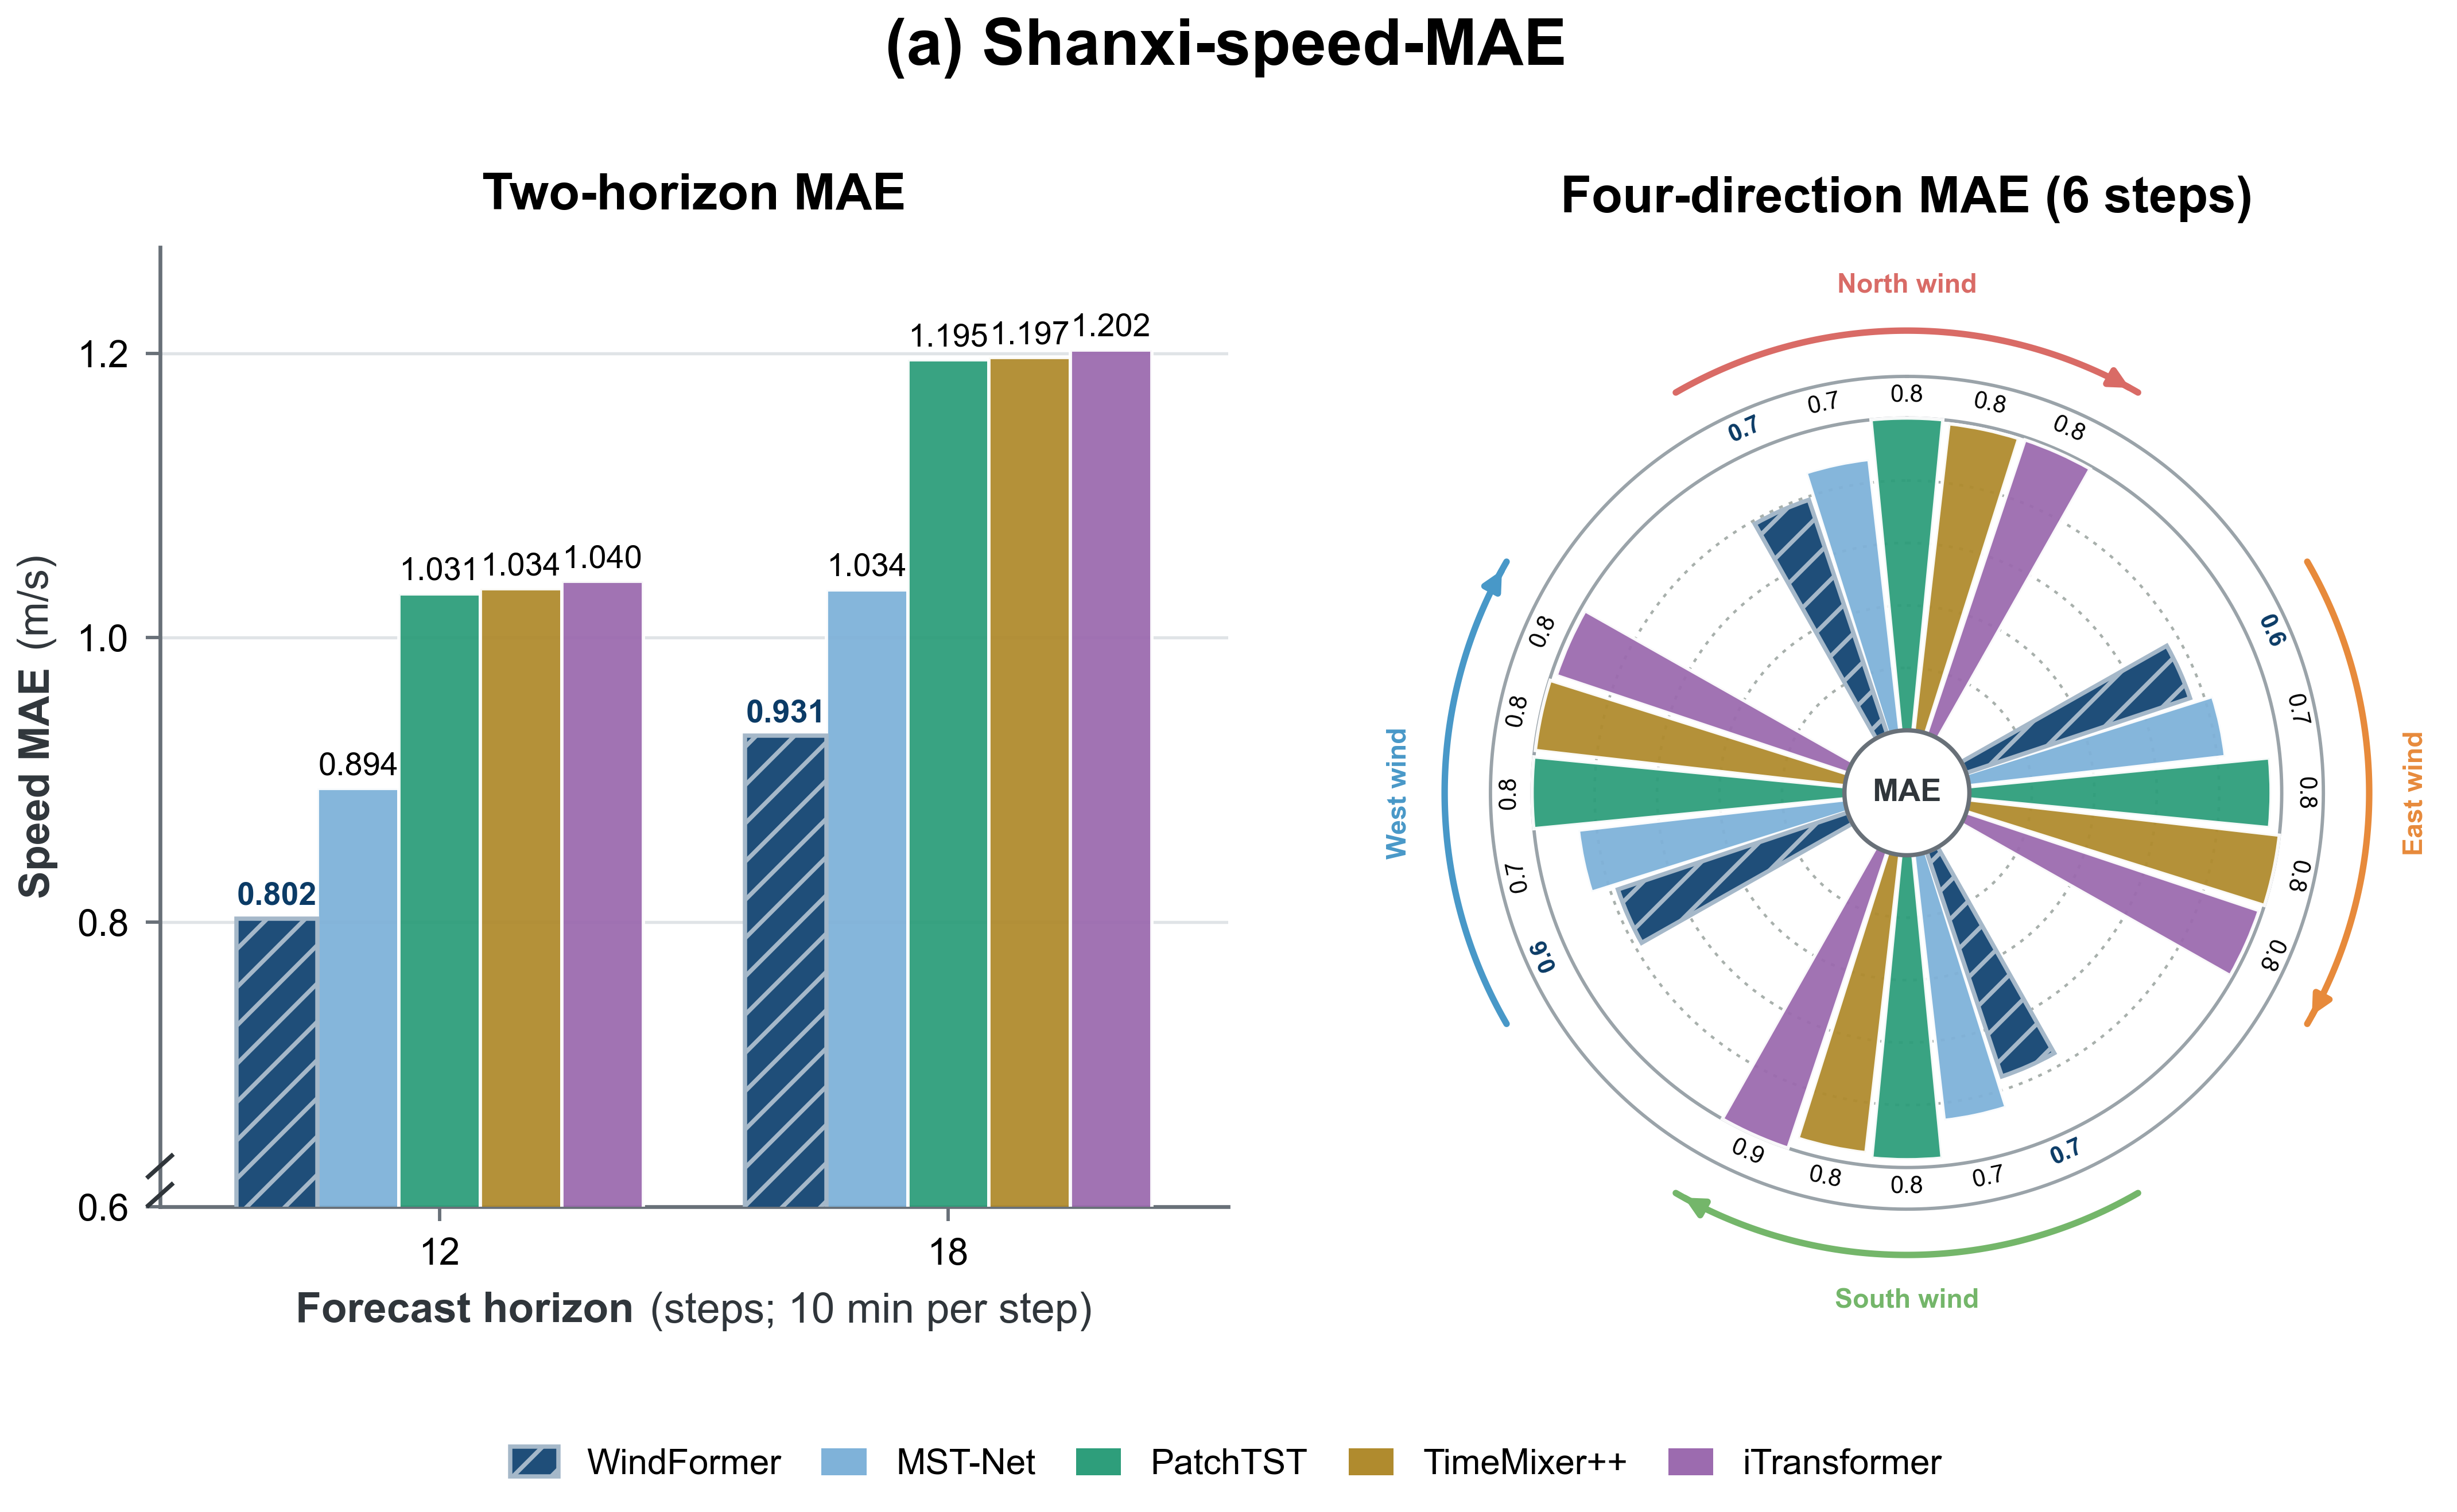
\includegraphics[width=0.49\textwidth]{figures/fig_shanxi_speed_mae.png} &
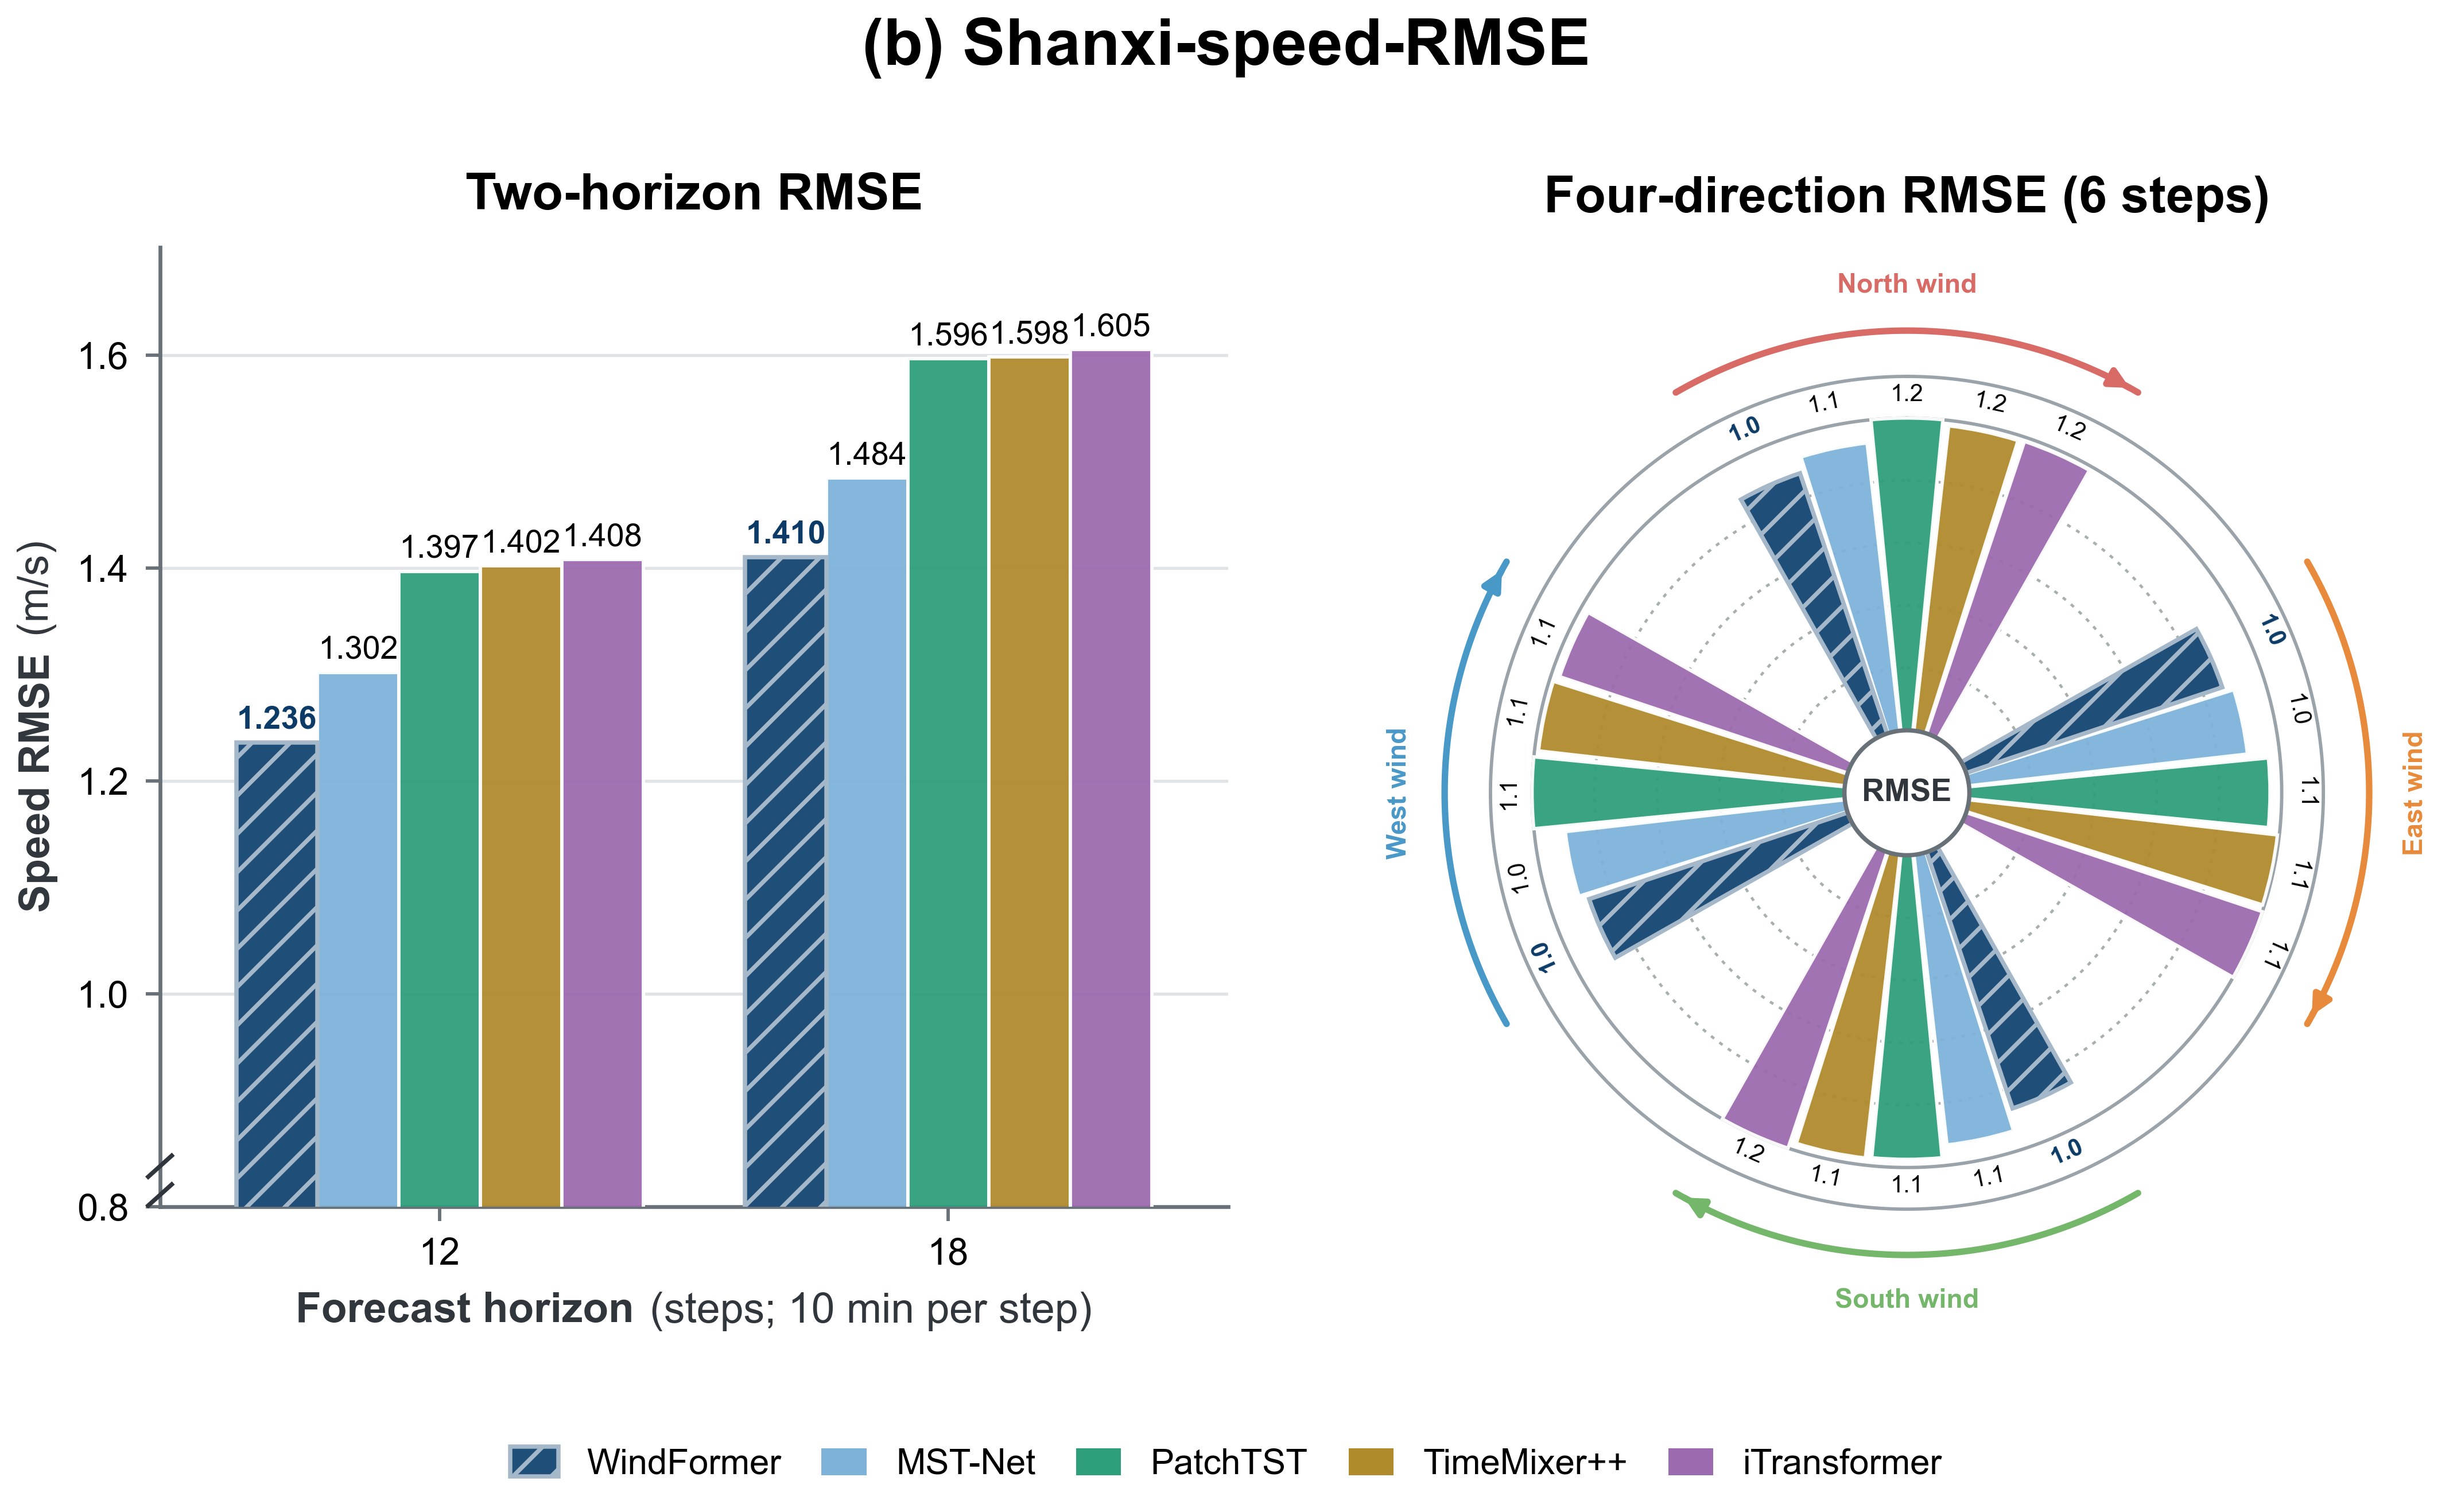
\includegraphics[width=0.49\textwidth]{figures/fig_shanxi_speed_rmse.png} \\[1pt]
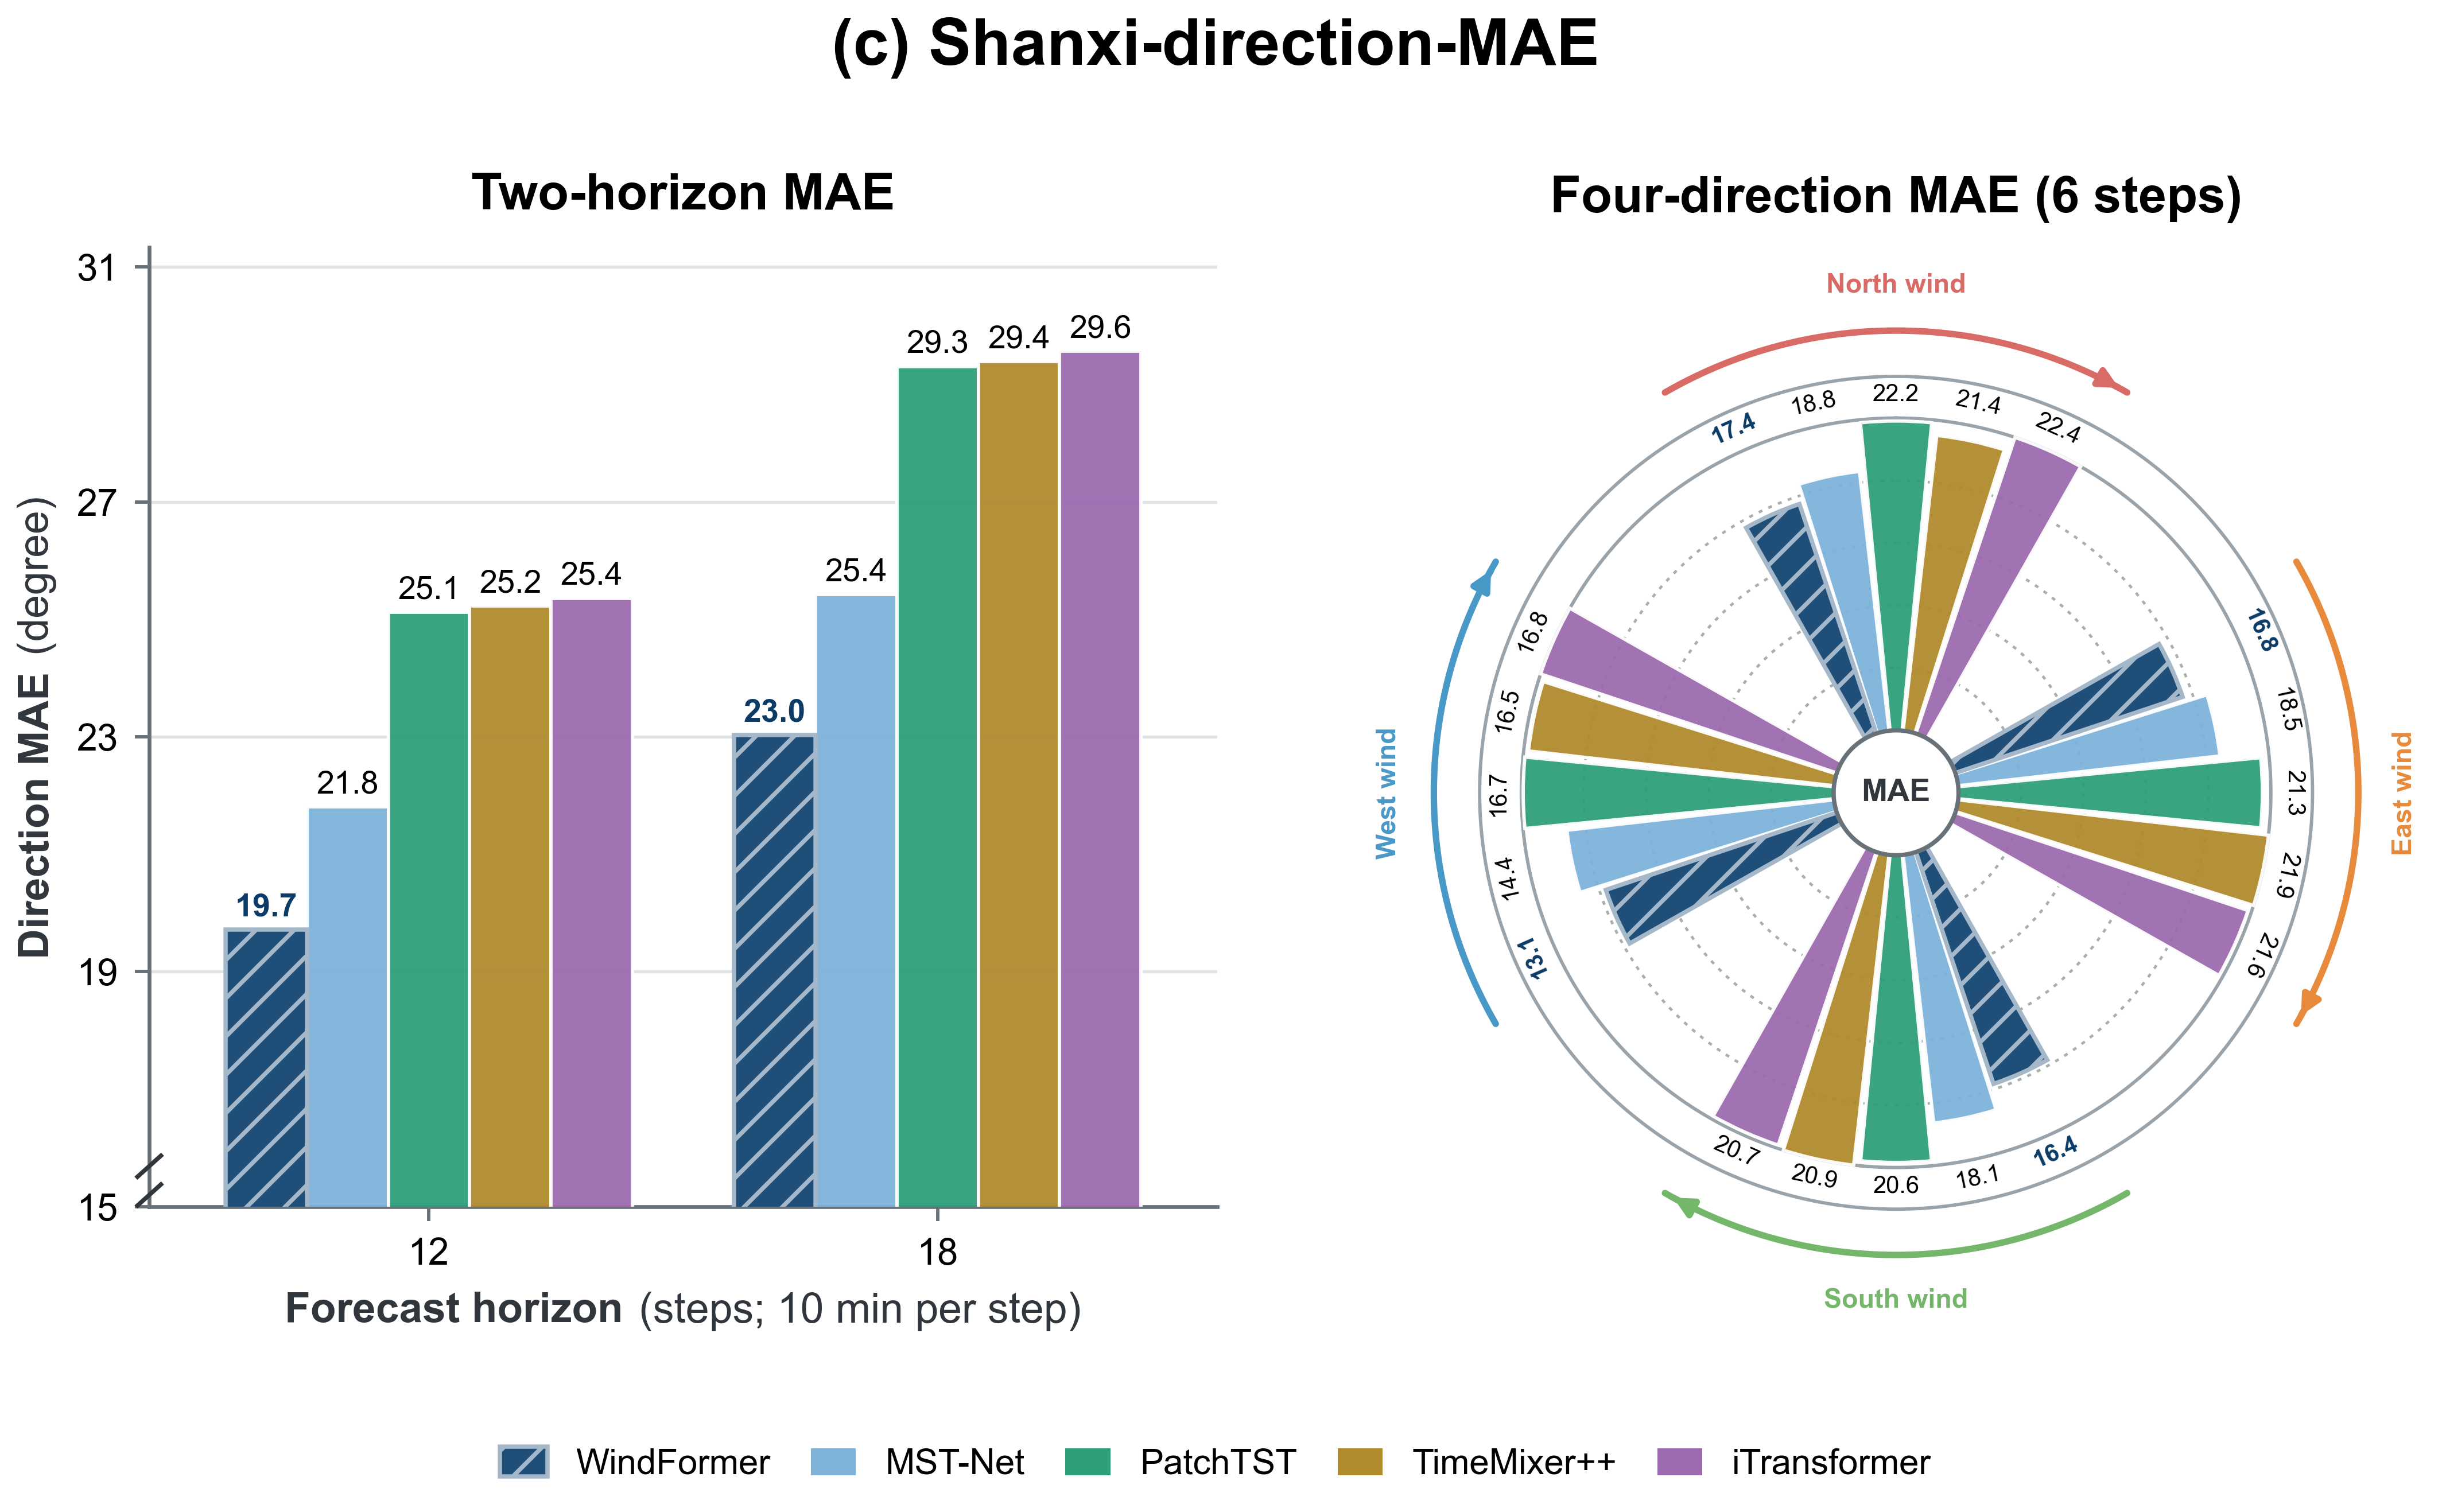
\includegraphics[width=0.49\textwidth]{figures/fig_shanxi_direction_mae.png} &
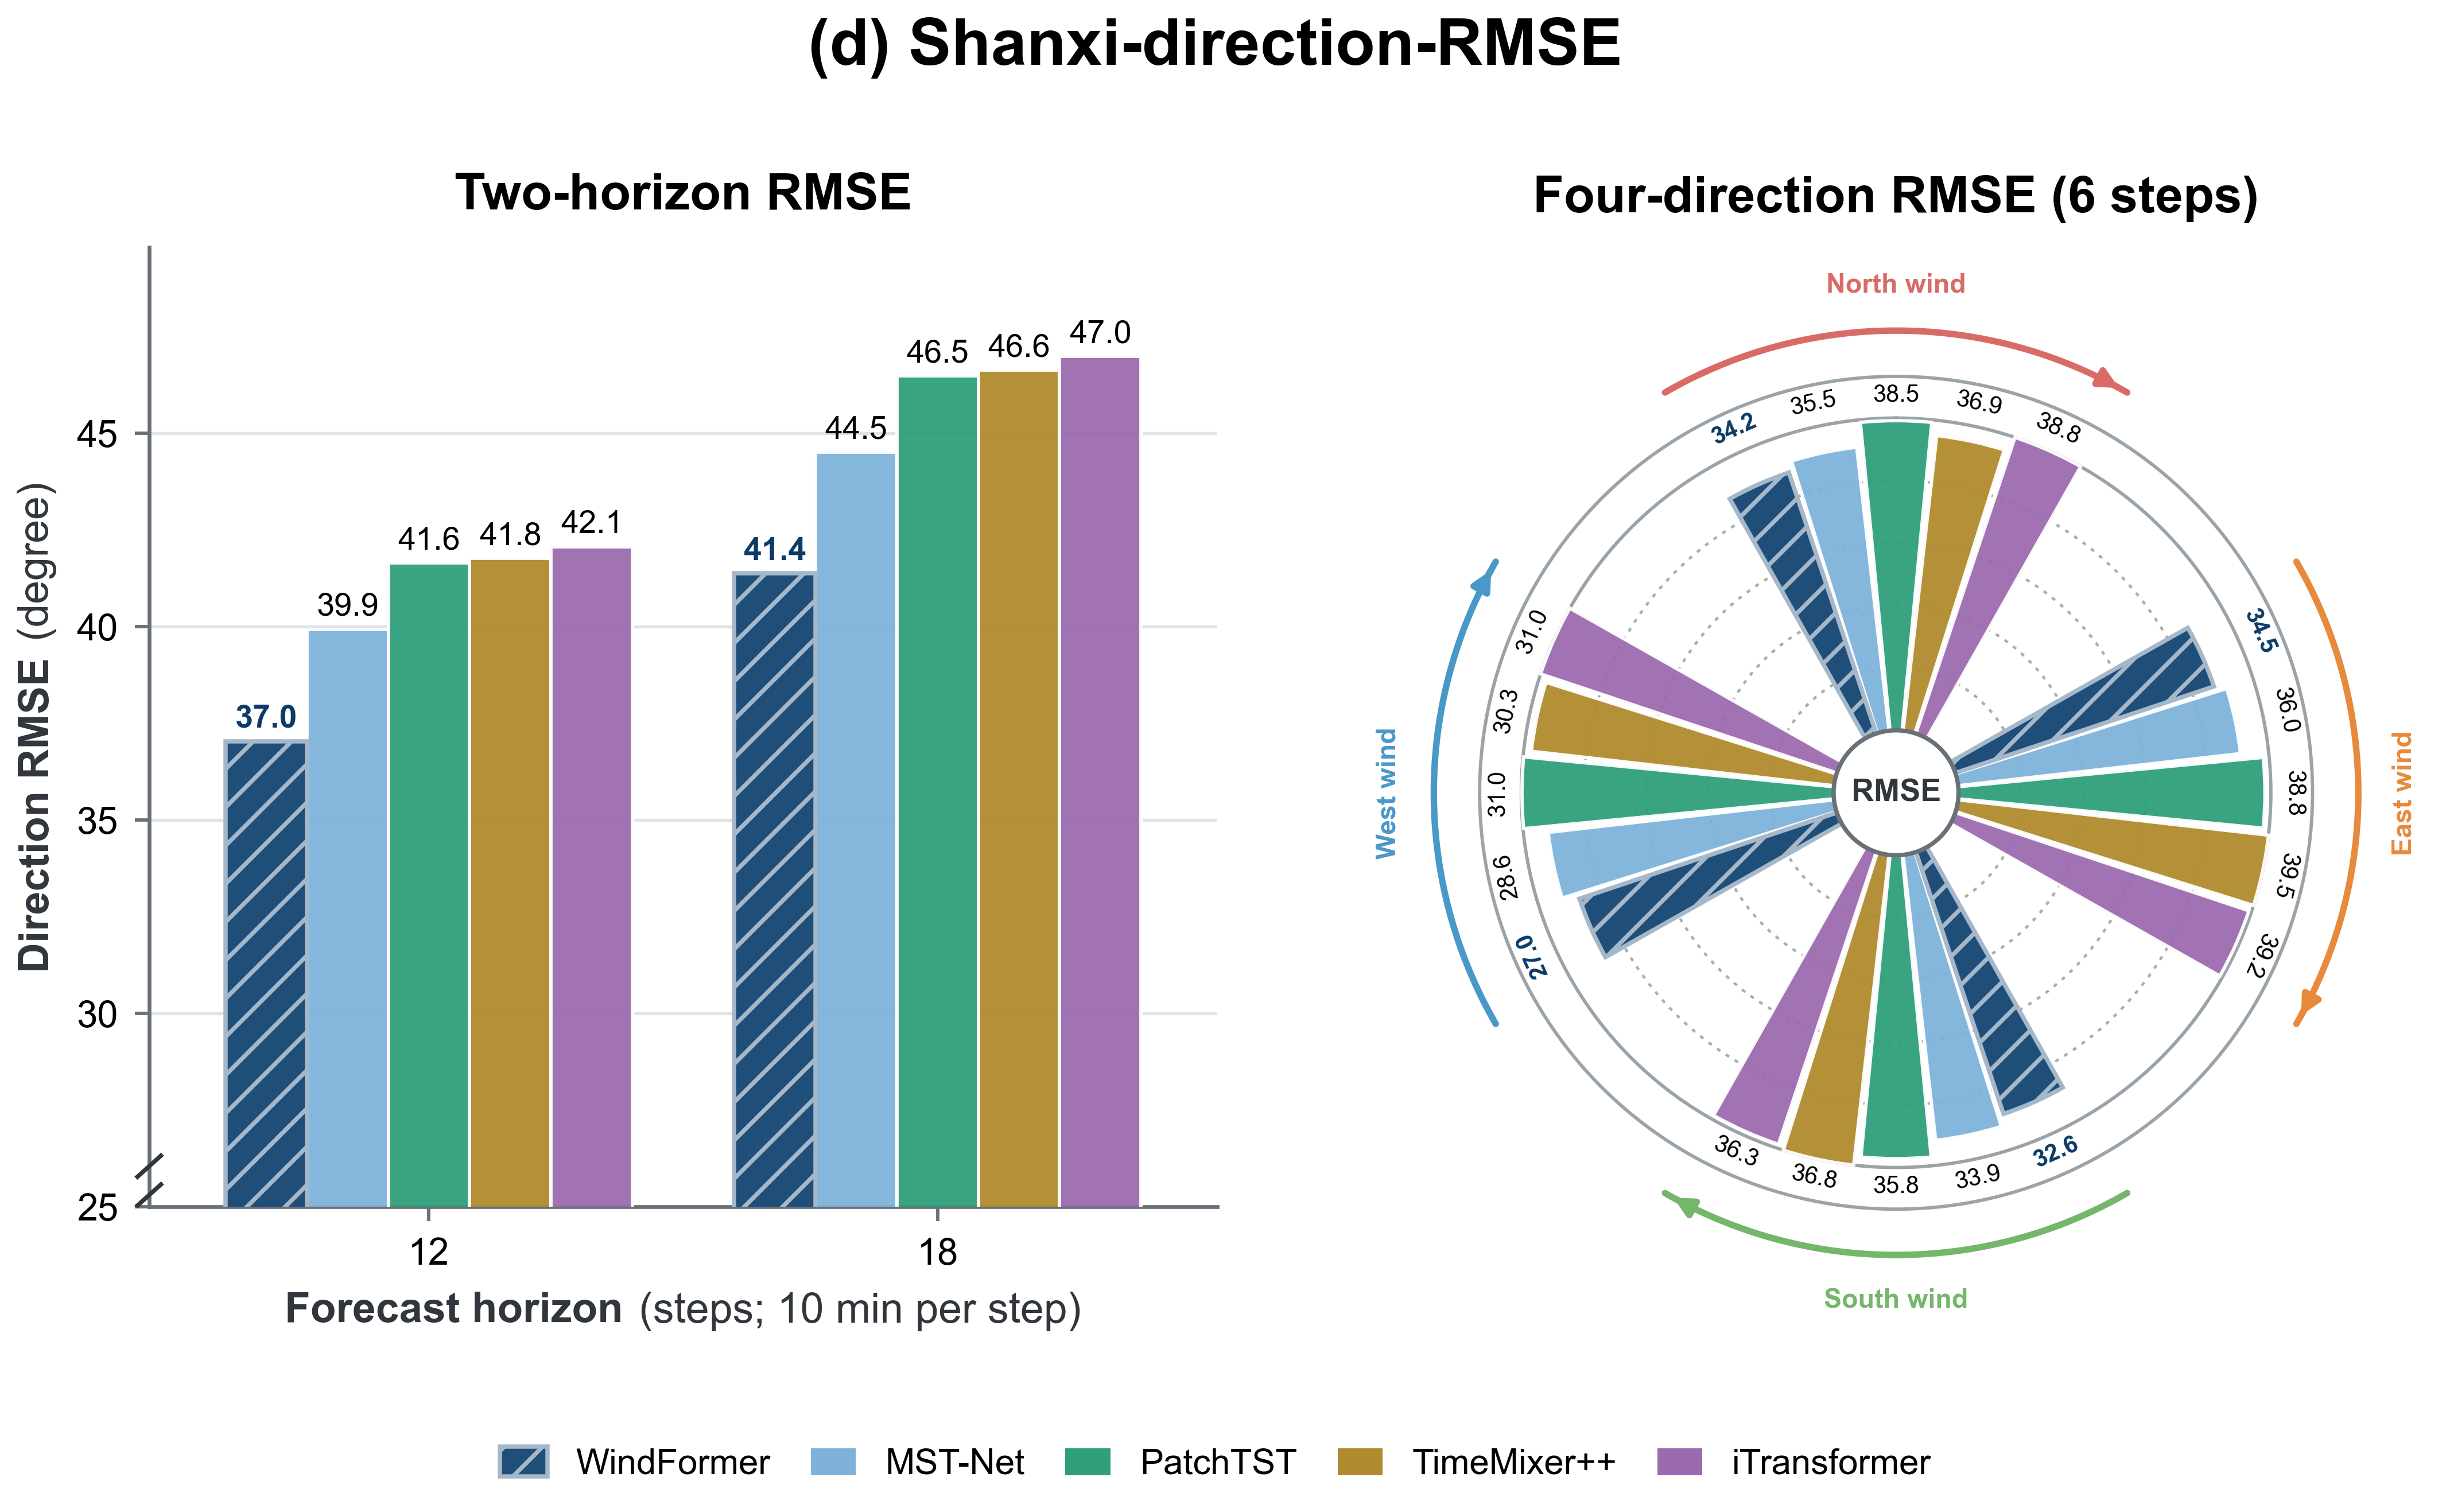
\includegraphics[width=0.49\textwidth]{figures/fig_shanxi_direction_rmse.png} \\[1pt]
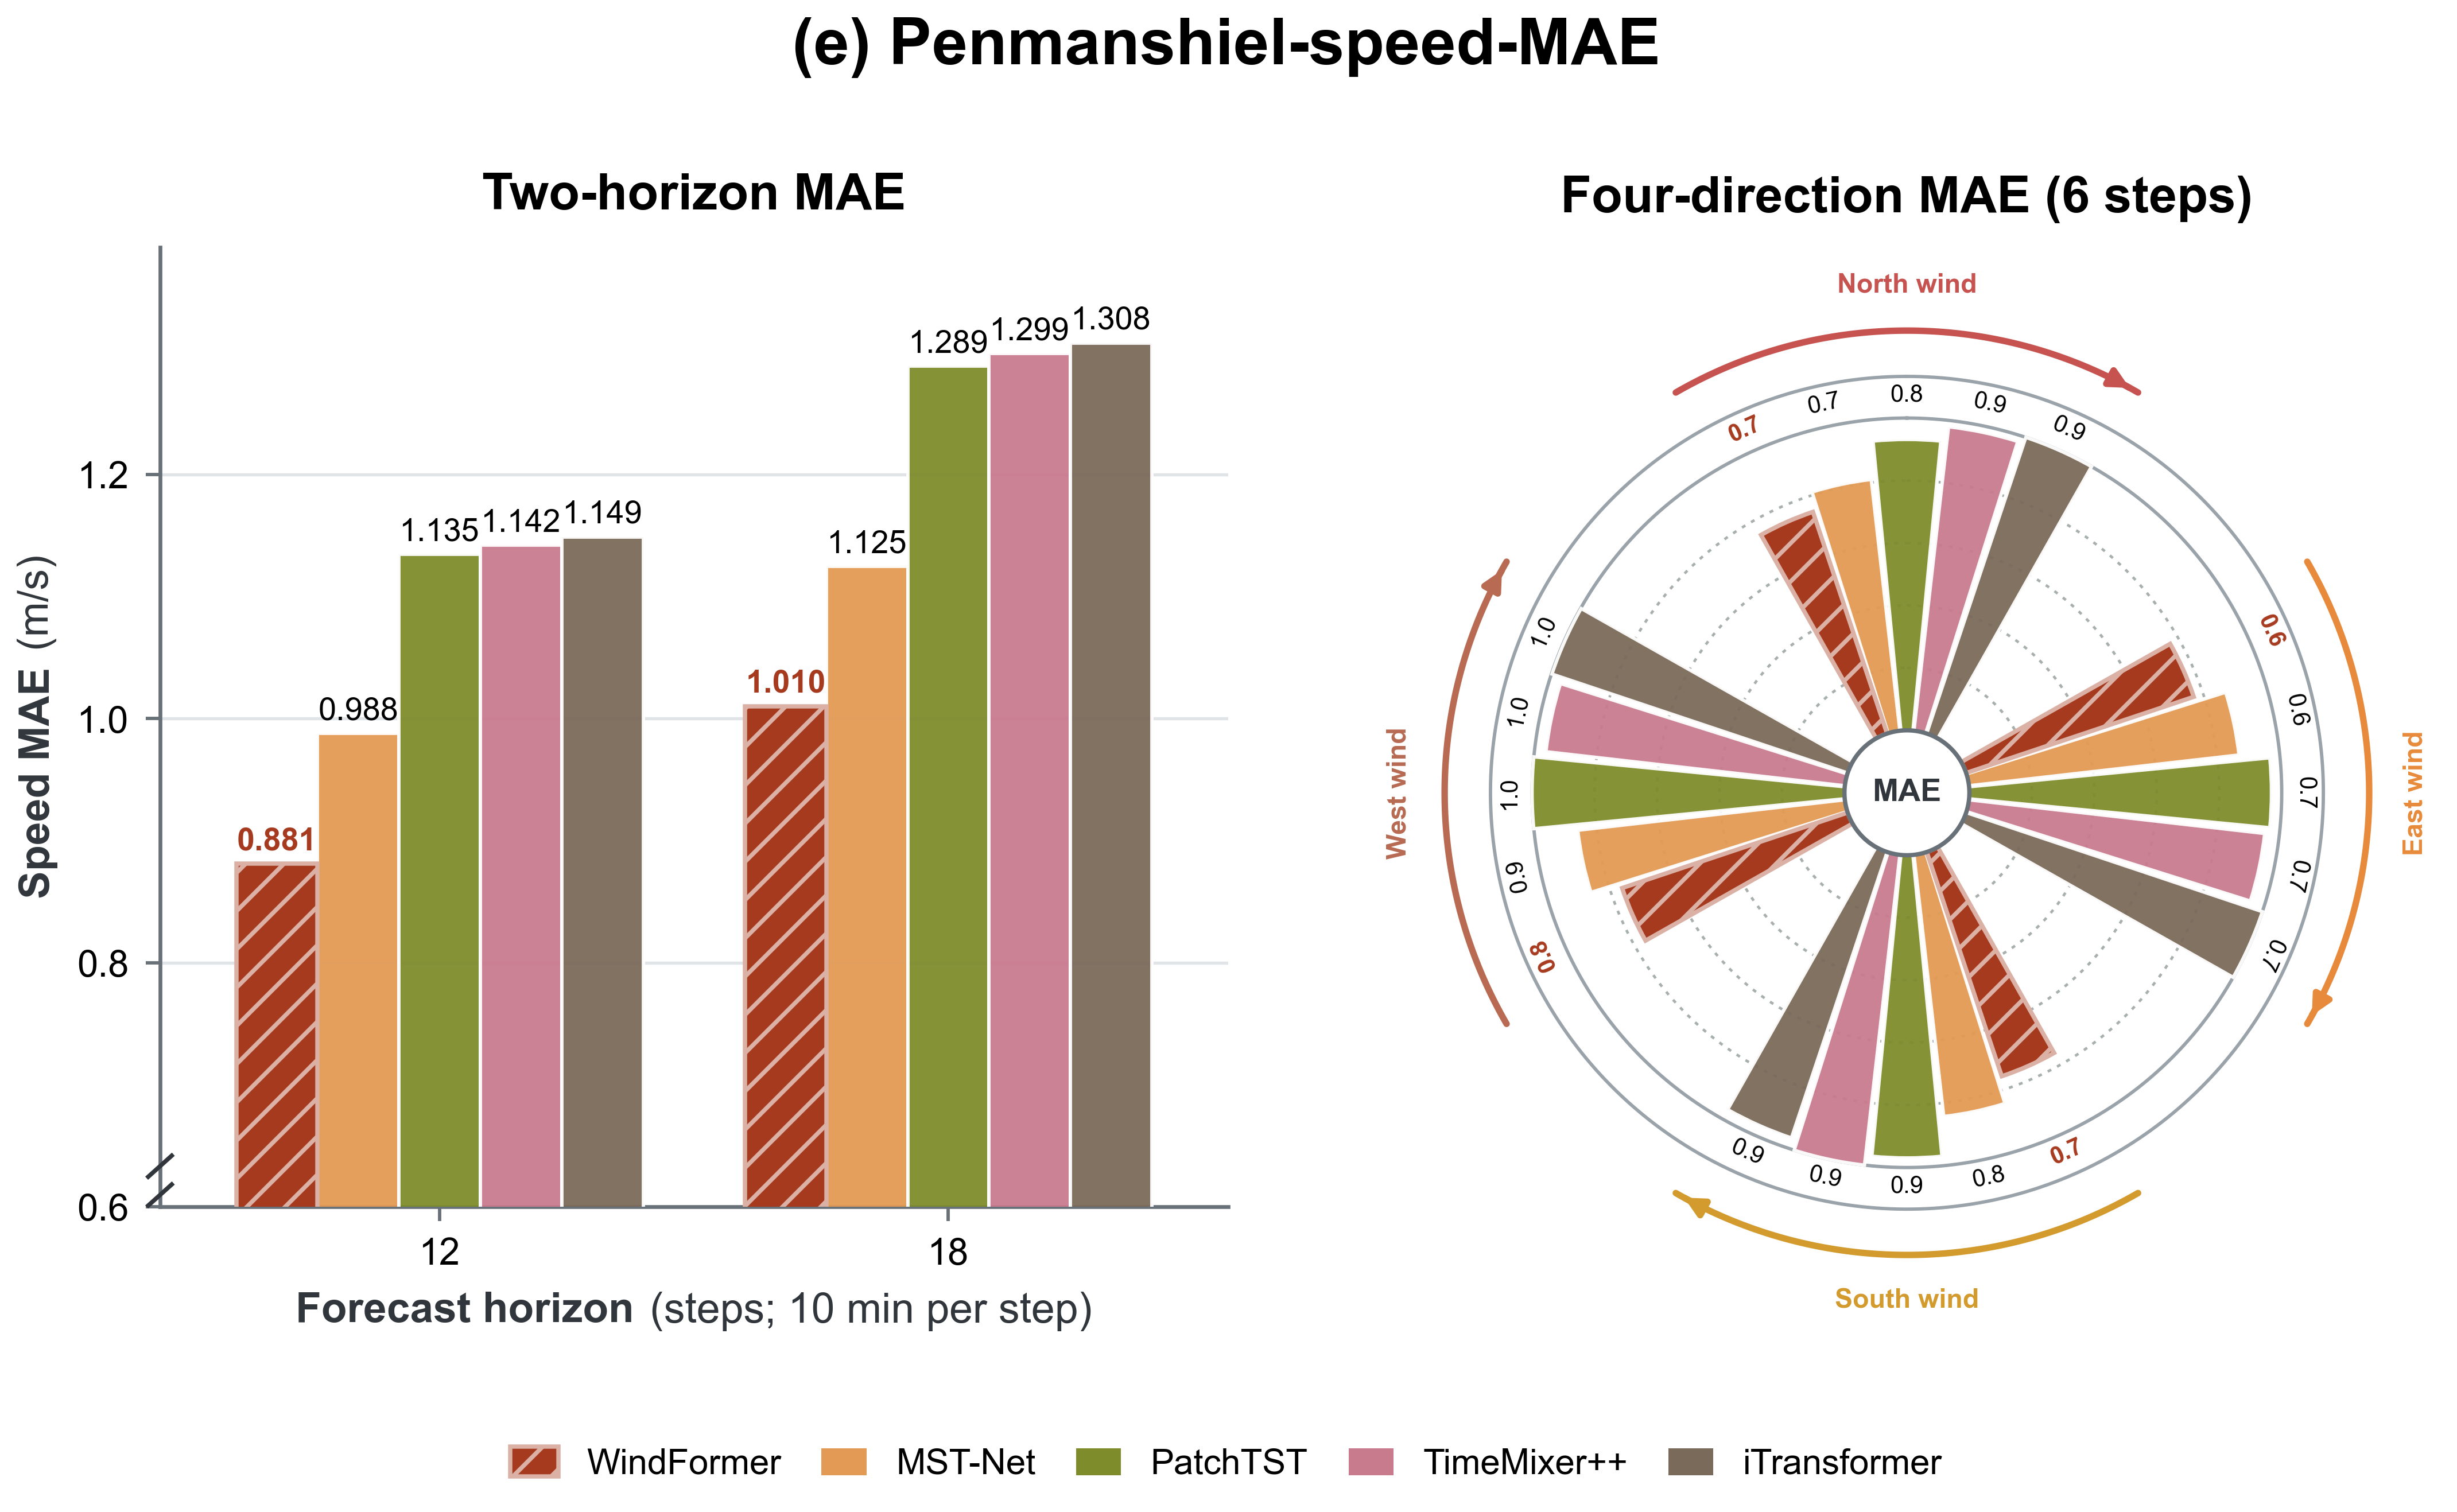
\includegraphics[width=0.49\textwidth]{figures/fig_penmanshiel_speed_mae.png} &
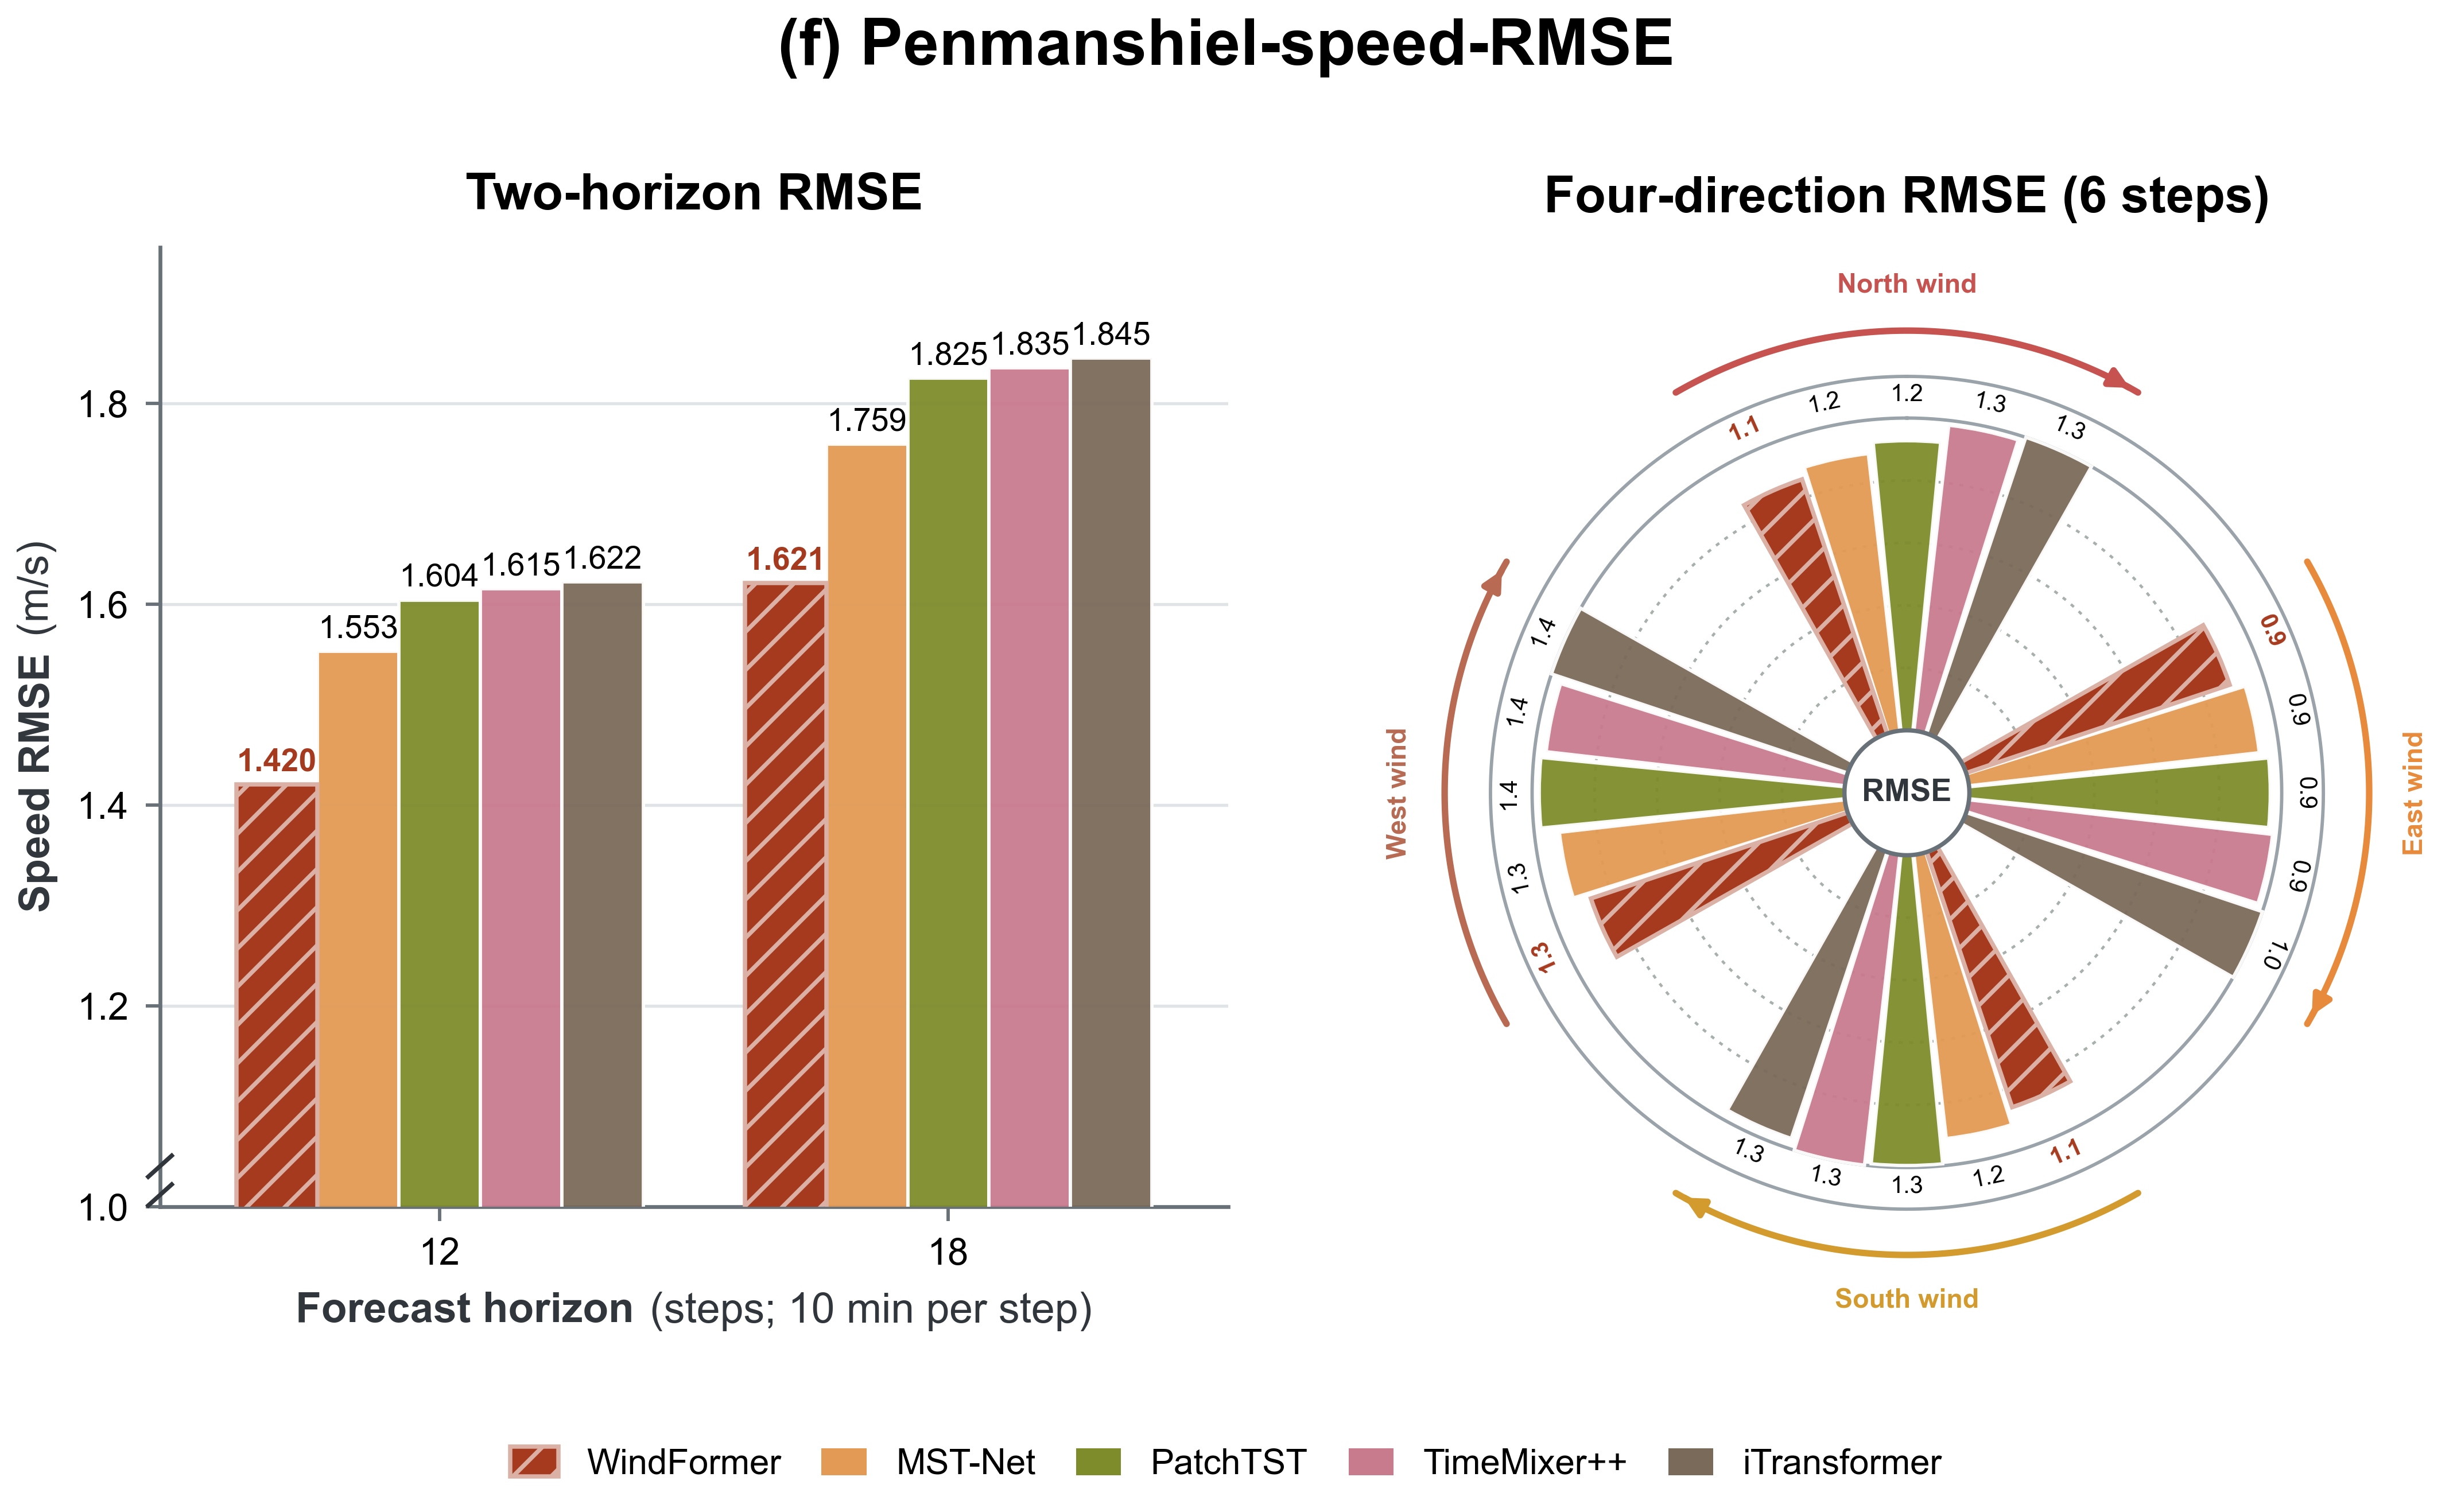
\includegraphics[width=0.49\textwidth]{figures/fig_penmanshiel_speed_rmse.png} \\[1pt]
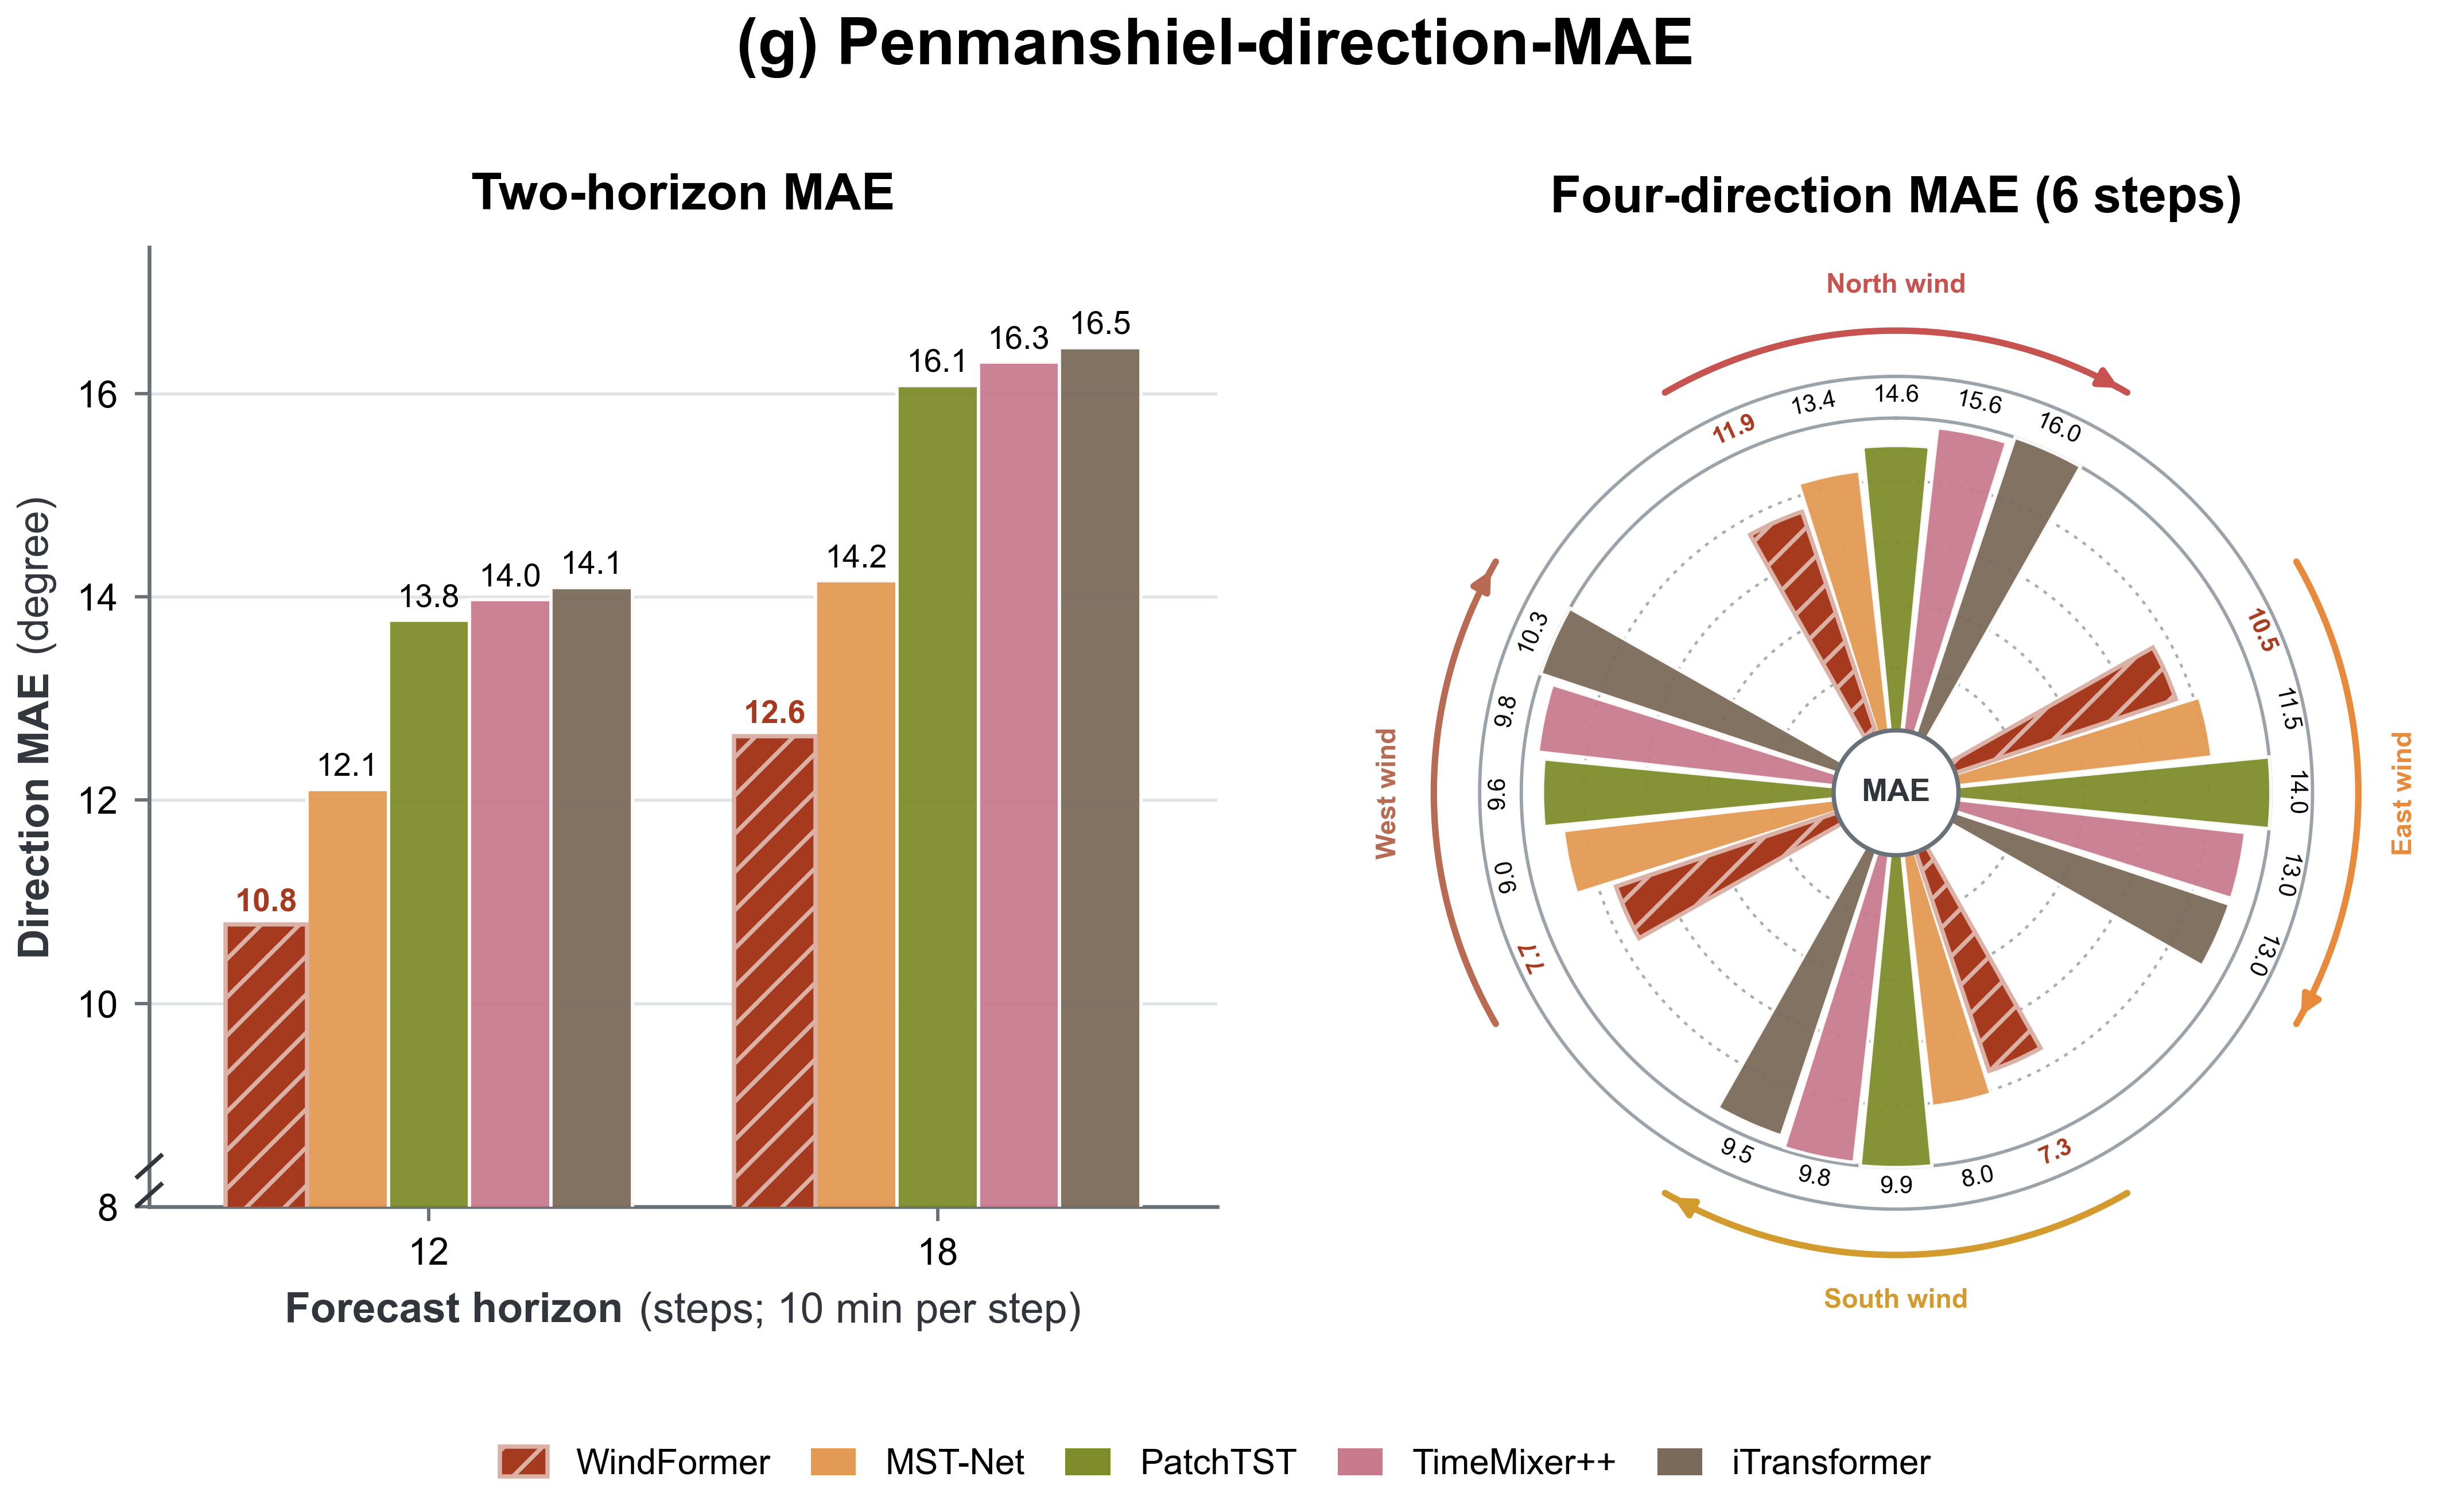
\includegraphics[width=0.49\textwidth]{figures/fig_penmanshiel_direction_mae.png} &
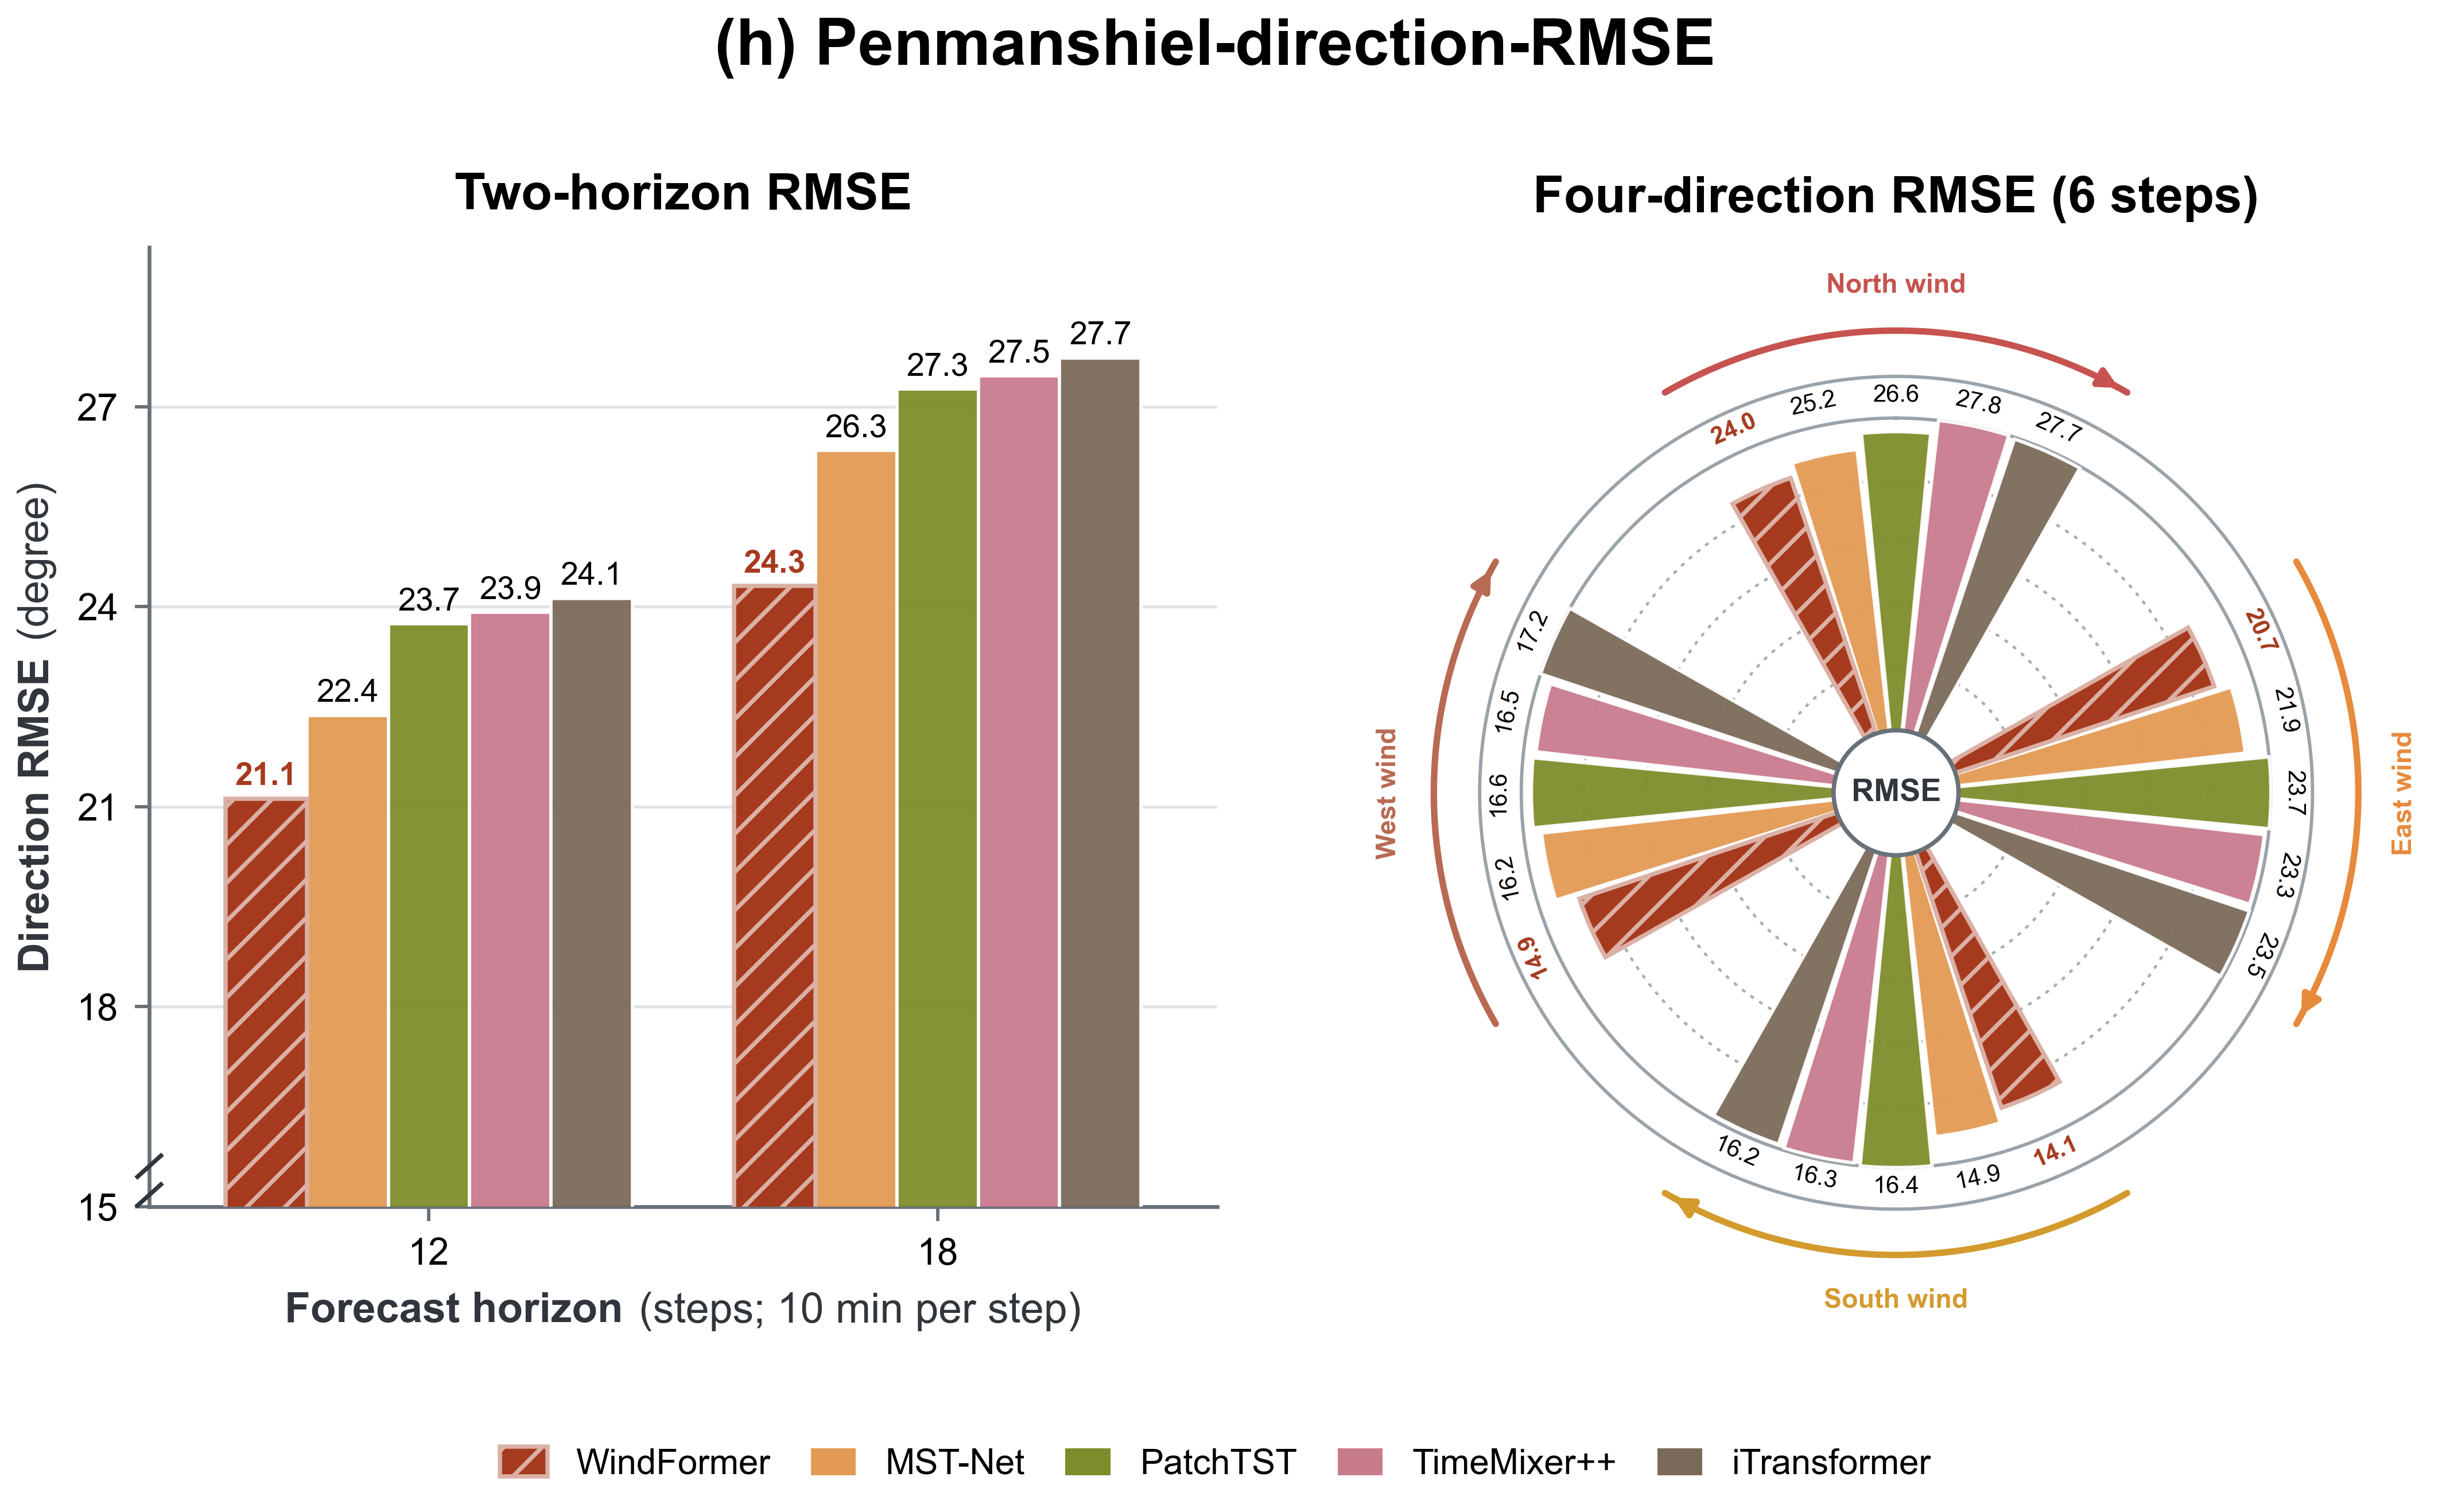
\includegraphics[width=0.49\textwidth]{figures/fig_penmanshiel_direction_rmse.png}
\end{tabular}
\vspace{-8pt}
\caption{Direction-aware forecasting results across the Shanxi and Penmanshiel wind farms. Each panel reports the two-horizon error comparison and four-direction error profile for one dataset--metric pair.}
\label{fig:formal_direction_aware_results}
\end{figure}

Figure~\ref{fig:formal_direction_aware_results} shows that the advantage is not restricted to a single aggregate score: the error profiles remain favorable across wind directions, wind variables, datasets, and reported metrics.

\begin{figure}[htbp]
\centering

\includegraphics[width=0.80\textwidth]{figures/result.png}
\caption{Representative 12-step full-sample prediction examples for wind speed and wind direction.}
\label{fig:prediction_examples}
\end{figure}

The representative forecasts in Fig.~\ref{fig:prediction_examples} further illustrate that WindFormer follows the shared trajectory while retaining turbine-level variation in the predicted signals.

\begin{table}[htbp]
\caption{Computational efficiency comparison at the 12-step forecasting horizon.}
\label{tab:efficiency}
\centering
\scriptsize
\setlength{\tabcolsep}{2.0pt}
\renewcommand{\arraystretch}{1.04}
\begin{adjustbox}{max width=\columnwidth}
\begin{tabular}{@{}lccccc@{}}
\toprule
Metric & WindFormer & MSGNet & PatchTST & iTransformer & TimeMixer++ \\
\midrule
Parameters & 36,512 & 26,680,000 & 140,492 & 124,428 & 388,332 \\
Train time (s) & 143.78 & 14356.30 & 315.32 & 57.80 & 109.55 \\
Peak GPU (MB) & 74.83 & 4532.1 & 3158.9 & 109.1 & 308.9 \\
\bottomrule
\end{tabular}
\end{adjustbox}
\end{table}

Table~\ref{tab:efficiency} shows that WindFormer combines the strongest forecasting results with a compact 36,512-parameter model and low peak GPU memory in the reported comparison.

The paired tests in Table~\ref{tab:paired-t-holm} compare WindFormer against MST-Net over five matched random seeds. All eight dataset--metric comparisons remain significant after Holm correction, supporting the consistency of the observed improvements rather than attributing them to a single seed.

\begin{table}[htbp]
\centering
\caption{Statistical significance of WindFormer improvements over MST-Net across five matched random seeds. Values are mean $\pm$ sample SD. The one-sided paired $t$-test evaluates whether WindFormer has lower error; $p_{\mathrm{raw}}$ and $p_{\mathrm{Holm}}$ are the raw and Holm-adjusted values across the eight dataset--metric comparisons.}
\label{tab:paired-t-holm}
\scriptsize
\setlength{\tabcolsep}{3.2pt}
\renewcommand{\arraystretch}{1.12}
\begin{adjustbox}{max width=\textwidth}
\begin{tabular}{clccrr}
\toprule
Dataset & Metric & WindFormer & MST-Net & $p_{\mathrm{raw}}$ & $p_{\mathrm{Holm}}$ \\
\midrule
\multirow[c]{4}{*}{Shanxi} & Speed MAE & 0.8025 $\pm$ 0.0048 & 0.8939 $\pm$ 0.0072 & $2.94\times 10^{-5}$ & $1.76\times 10^{-4}$\\
& Speed RMSE & 1.2374 $\pm$ 0.0074 & 1.3033 $\pm$ 0.0105 & $4.22\times 10^{-4}$ & $6.60\times 10^{-4}$\\
& Direction MAE & 0.3441 $\pm$ 0.0027 & 0.3806 $\pm$ 0.0038 & $3.56\times 10^{-5}$ & $1.76\times 10^{-4}$\\
& Direction RMSE & 0.6525 $\pm$ 0.0052 & 0.7041 $\pm$ 0.0070 & $3.30\times 10^{-4}$ & $6.60\times 10^{-4}$\\
\addlinespace
\multirow[c]{4}{*}{Penmanshiel} & Speed MAE & 0.8812 $\pm$ 0.0053 & 0.9879 $\pm$ 0.0078 & $3.02\times 10^{-6}$ & $2.41\times 10^{-5}$\\
& Speed RMSE & 1.4211 $\pm$ 0.0085 & 1.5538 $\pm$ 0.0124 & $1.73\times 10^{-5}$ & $1.21\times 10^{-4}$\\
& Direction MAE & 0.1881 $\pm$ 0.0015 & 0.2113 $\pm$ 0.0021 & $3.48\times 10^{-5}$ & $1.76\times 10^{-4}$\\
& Direction RMSE & 0.3686 $\pm$ 0.0030 & 0.3905 $\pm$ 0.0039 & $1.46\times 10^{-4}$ & $4.37\times 10^{-4}$\\
\bottomrule
\end{tabular}
\end{adjustbox}
\end{table}


Together, these results answer RQ1 affirmatively. WindFormer improves accuracy across both wind variables and datasets while remaining computationally compact and statistically consistent across matched seeds.

\subsection{RQ2: Which Structural Components Drive the Improvements?}
\label{subsec:ablation}

RQ2 examines whether the gains are attributable to the components introduced for the two challenges rather than to model capacity alone. The ablations therefore remove the learnable common-field weights, the circular direction representation, the wind-vector consistency loss, or the Phase-Attention temporal organization.

\begin{table}[htbp]
\caption{Ablation study results for different variants on the Shanxi and Penmanshiel datasets.}
\label{tab:ablation}
\centering
\scriptsize
\setlength{\tabcolsep}{3.2pt}
\renewcommand{\arraystretch}{1.08}
\begin{adjustbox}{max width=\textwidth}
\begin{tabular}{l|cccc|cccc|cccc|cccc}
\toprule
\multirow{3}{*}{Variant}
& \multicolumn{4}{c|}{Shanxi-6steps}
& \multicolumn{4}{c|}{Shanxi-12steps}
& \multicolumn{4}{c|}{Penmanshiel-6steps}
& \multicolumn{4}{c}{Penmanshiel-12steps} \\
\cline{2-17}
& \multicolumn{2}{c}{Speed} & \multicolumn{2}{c|}{Wdir}
& \multicolumn{2}{c}{Speed} & \multicolumn{2}{c|}{Wdir}
& \multicolumn{2}{c}{Speed} & \multicolumn{2}{c|}{Wdir}
& \multicolumn{2}{c}{Speed} & \multicolumn{2}{c}{Wdir} \\
\cline{2-17}
& MAE & RMSE & MAE & RMSE
& MAE & RMSE & MAE & RMSE
& MAE & RMSE & MAE & RMSE
& MAE & RMSE & MAE & RMSE \\
\midrule
WindFormer
& \textbf{0.6367} & \textbf{0.9884} & \textbf{0.2717} & \textbf{0.5530}
& \textbf{0.8025} & \textbf{1.2374} & \textbf{0.3441} & \textbf{0.6525}
& \textbf{0.7142} & \textbf{1.1497} & \textbf{0.1456} & \textbf{0.2914}
& \textbf{0.8812} & \textbf{1.4211} & \textbf{0.1881} & \textbf{0.3686} \\
w/o Learnable Weights
& 0.6754 & 1.0421 & 0.2765 & 0.5601
& 0.8465 & 1.3012 & 0.3495 & 0.6612
& 0.7589 & 1.2185 & 0.1502 & 0.2985
& 0.9325 & 1.5052 & 0.1935 & 0.3768 \\
w/o Direction Vector Rep.
& 0.6502 & 1.0065 & 0.6214 & 1.0851
& 0.8188 & 1.2615 & 0.7245 & 1.2562
& 0.7285 & 1.1712 & 0.4985 & 0.8124
& 0.8985 & 1.4485 & 0.5642 & 0.9351 \\
w/o Wind Vector Cons.
& 0.6612 & 1.0215 & 0.2985 & 0.5921
& 0.8315 & 1.2825 & 0.3852 & 0.7124
& 0.7412 & 1.1921 & 0.1685 & 0.3341
& 0.9125 & 1.4721 & 0.2185 & 0.4215 \\
Phase-Attn to Patch
& 0.6845 & 1.0563 & 0.2798 & 0.5644
& 0.8582 & 1.3155 & 0.3541 & 0.6658
& 0.7695 & 1.2312 & 0.1534 & 0.3018
& 0.9458 & 1.5215 & 0.1972 & 0.3812 \\
\bottomrule
\end{tabular}
\end{adjustbox}
\end{table}

Table~\ref{tab:ablation} supports the intended division of labor. Removing the direction-vector representation mainly harms direction prediction, whereas removing the learnable common-field weights or replacing Phase-Attention with ordinary patches affects wind-speed prediction more strongly. Removing the wind-vector consistency term degrades both tasks, consistent with its role as the objective-level coupling between the two branches.

\subsection{Hyperparameter Sensitivity Analysis}
\label{subsec:hyperparameter_sensitivity}

We further evaluate the sensitivity of WindFormer to four capacity and receptive-field choices: the historical input window length, the Phase Token projection dimension, the hidden dimension of the shared residual MLP, and the number of direction-branch Transformer layers. The results are summarized in Fig.~\ref{fig:hyperparameter_sensitivity}. Across all four metrics, the default configuration remains close to the best-performing setting, indicating that the structural design is not dependent on a narrow hyperparameter choice.

\begin{figure}[htbp]
\centering

\includegraphics[width=0.82\textwidth]{figures/hyperparameter_sensitivity.png}
\caption{Hyperparameter sensitivity analysis on the Shanxi dataset. The four panels vary the historical window length, Phase Token projection dimension, shared residual MLP width, and direction-branch Transformer depth.}
\label{fig:hyperparameter_sensitivity}
\end{figure}

These results answer RQ2 by linking each component to the challenge it was designed to address, while showing that the complete model does not depend on a single finely tuned capacity setting.

\subsection{RQ3: Is WindFormer Robust under Noisy and Extreme Conditions?}
\label{subsec:robustness}

RQ3 evaluates whether the structure-aware design remains useful when the inputs deviate from the clean training distribution. We consider sensor perturbations and increasing extreme-volatility severity.

For sensor perturbation, let $\theta_{i,t}$ denote the wind direction of turbine $i$ at time $t$, and let $\mathcal{W}(\cdot)$ wrap angles to the valid range. Only the wind-direction channel in the training inputs is corrupted as
\begin{equation}
\tilde{\theta}_{i,t}^{(\sigma)}=\mathcal{W}\left(\theta_{i,t}+\epsilon_{i,t}^{(\sigma)}\right),\quad
\epsilon_{i,t}^{(\sigma)}\sim\mathcal{N}(0,\sigma^2),
\label{eq:sensor_noise}
\end{equation}
where $\sigma\in\{0.1,0.2,0.3\}$ rad. Test inputs and labels remain unchanged, and all models are retrained at each noise level.

\begin{figure}[htbp]
\centering

\includegraphics[width=0.80\textwidth]{figures/supp_sensor_robustness.png}
\caption{Sensor Perturbation Robustness. The comparison covers all models, both wind speed and wind direction, and both datasets. Each subplot uses its own vertical scale to preserve dataset-specific variation.}
\label{fig:sensor_perturbation}
\end{figure}

The second experiment evaluates gust-like transient fluctuations through an EVT-inspired residual stratification scheme \cite{Pickands1975StatisticalInferenceUsingExtremeOrderStatistics,Cleveland1990STLSeasonalTrendDecomposition}. For a target series $y_t$, seasonal-trend decomposition using LOESS gives
\begin{equation}
y_t=T_t+S_t+R_t,
\end{equation}
where $T_t$, $S_t$, and $R_t$ denote the trend, seasonal, and residual terms, respectively. The extreme threshold is estimated only from the training split:
\begin{equation}
u=Q_{0.99}\left(\{|R_t|:t\in\mathcal{T}_{\mathrm{train}}\}\right),
\end{equation}
where $Q_{0.99}(\cdot)$ is the 99th percentile. A time step is identified as an extreme event when
\begin{equation}
I_t=\mathbb{I}(|R_t|>u).
\end{equation}
Given an input window of length $L=288$ ending at time $t$, the volatility severity of the corresponding forecasting sample is quantified by
\begin{equation}
N_{\mathrm{extreme}}(t)=\sum_{\tau=t-L+1}^{t}I_{\tau}.
\end{equation}
Test samples are binned by $N_{\mathrm{extreme}}(t)$ and evaluated with the trained model held fixed.

\begin{figure}[htbp]
\centering

\includegraphics[width=0.80\textwidth]{figures/supp_extreme_stress.png}
\caption{Extreme Volatility Stress Test on the Penmanshiel dataset. The figure reports wind speed and wind direction errors under increasing values of $N_{\mathrm{extreme}}$.}
\label{fig:extreme_stress}
\end{figure}

Figures~\ref{fig:sensor_perturbation} and \ref{fig:extreme_stress} show that WindFormer experiences the smallest degradation under both sensor noise and increasing extreme residual severity. This suggests that separating shared dynamics from local variation and respecting directional geometry remains beneficial when the input distribution is perturbed.

These results answer RQ3 affirmatively: WindFormer retains a more stable error profile as measurement noise and transient volatility increase.

\subsection{RQ4: Can WindFormer Generalize to Unseen Turbines?}
\label{subsec:zero_shot}

RQ4 tests whether the shared temporal parameters can transfer beyond the turbines observed during training. We conduct the \emph{Sparse Deployment Zero-Shot Evaluation} on Penmanshiel. Let $\mathcal{V}$ denote all turbines and $\mathcal{S}_k\subset\mathcal{V}$ the four turbines randomly selected in trial $k$. The remaining turbines
\begin{equation}
\mathcal{U}_k=\mathcal{V}\setminus\mathcal{S}_k
\end{equation}
are treated as unseen zero-shot targets. For a model $f_{\phi}$, $\phi$ is trained only on $\mathcal{D}_{\mathrm{train}}(\mathcal{S}_k)$ and evaluated on $\mathcal{D}_{\mathrm{test}}(\mathcal{U}_k)$. The reported error is averaged over three independent trials:
\begin{equation}
\mathrm{Err}_{\mathrm{ZS}}=\frac{1}{3}\sum_{k=1}^{3}\mathrm{Err}\left(f_{\phi_k},\mathcal{D}_{\mathrm{test}}(\mathcal{U}_k)\right).
\end{equation}
Three conditions are compared: full-sample training, zero-shot transfer, and zero-shot transfer with 0.3-rad angular noise.

\begin{figure}[htbp]
\centering

\includegraphics[width=0.80\textwidth]{figures/supp_sparse_zero_shot.png}
\caption{Sparse Deployment Zero-Shot Evaluation on Penmanshiel. The figure compares full-sample training, zero-shot transfer, and zero-shot transfer under sensor noise across multiple forecast horizons.}
\label{fig:sparse_zero_shot}
\end{figure}

Figure~\ref{fig:sparse_zero_shot} shows that WindFormer has the smallest zero-shot degradation, with a 17.72\% increase in direction MAE under the clean setting and a 15.61\% increase under 0.3-rad noise. The result indicates that shared temporal parameters and geometry-aware direction modeling can transfer to turbines that were not used as training targets.

Thus, RQ4 is answered affirmatively. WindFormer provides the strongest cross-turbine transfer among the compared models under the tested sparse-deployment conditions.


\section{Conclusion}
\label{sec:conclusion}
This paper presented WindFormer as a structure-aware framework for joint short-term forecasting of wind speed and wind direction in multi-turbine wind farms. Its central design principle is to share information where it is physically common and preserve information where it is turbine-specific: the wind-speed branch separates a learnable common field from local residuals and organizes the common history with Phase-Attention over screened candidate temporal scales, while the wind-direction branch retains turbine-wise sequences in a continuous sine-cosine space. A wind-vector consistency objective couples the two representation-decoupled branches during training.

The experiments answer the four research questions in sequence. WindFormer improves standard wind-speed and wind-direction forecasting across both public wind farms and remains computationally compact. The ablations show that the common-field weights, phase-aware temporal organization, circular direction representation, and vector-consistency loss contribute to the corresponding aspects of the performance. Perturbation and extreme-volatility tests show more stable degradation, while sparse-deployment experiments indicate transfer to unseen turbines. These findings support the broader conclusion that multi-turbine wind forecasting benefits from matching the model representation to the physical structure of each wind variable rather than applying one homogeneous interaction pattern to all channels.

The current study focuses on SCADA-based short-term forecasting and does not introduce a geographic graph correction in the final WindFormer configuration. Future work can investigate adaptive geographic or wake-aware extensions while retaining the same principle of separating shared dynamics from turbine-specific information.

\bibliographystyle{elsarticle-num}
\bibliography{references}

\end{document}
